\chapter{Optimization}

Optimization pervades chemical engineering. Engineers use it to estimate reaction rate constants from data, to design efficient processes, to determine optimal control actions, to calculate thermodynamic equilibrium by minimizing Gibbs free energy, to train machine learning models by adjusting their parameters for greater accuracy, and much more.

In any optimization problem, we define the variables that can be changed, specify the objective we want to achieve, and then search for the conditions that yield the best performance, either a maximum or a minimum. This chapter introduces the foundations of optimization and the numerical methods used to solve these problems.

\section{Preliminaries: Gradients, Hessians, and Taylor Expansions}
Let's refresh our memory on some important concepts from calculus that will be used throughout this chapter. For a differentiable $f: \mathbb{R}^N \to \mathbb{R}$ and $\mathbf{x} = (x_1,\dots,x_N)^\top$, the gradient evaluated at $\mathbf{x}^*$ is
\begin{equation}
    \renewcommand{\arraystretch}{1.5}
    \nabla f(\mathbf{x}^*) = \begin{bmatrix}
        \frac{\partial f}{\partial x_1}(\mathbf{x}^*) \\
        \frac{\partial f}{\partial x_2}(\mathbf{x}^*) \\
        \vdots \\
        \frac{\partial f}{\partial x_N}(\mathbf{x}^*)
    \end{bmatrix}
    \end{equation}
The Hessian evaluated at $\mathbf{x}^*$ is
\begin{equation}
    \renewcommand{\arraystretch}{1.5}
    \nabla^2 f(\mathbf{x}^*) = \begin{bmatrix}
        \frac{\partial^2 f}{\partial x_1\partial x_1}(\mathbf{x}^*) & \cdots & \frac{\partial^2 f}{\partial x_1\partial x_N}(\mathbf{x}^*) \\
        \vdots & \ddots & \vdots \\
        \frac{\partial^2 f}{\partial x_N\partial x_1}(\mathbf{x}^*) & \cdots & \frac{\partial^2 f}{\partial x_N\partial x_N}(\mathbf{x}^*)
    \end{bmatrix}
\end{equation}
If all mixed partial derivatives are continuous in a neighborhood of $\mathbf{x}$, then $\nabla^2 f(\mathbf{x})$ is symmetric.

For univariate $f: \mathbb{R} \to \mathbb{R}$, if $f$ has a continuous second derivative in a neighborhood of $x^*$, a first-order Taylor expansion at $x^*$ is
\begin{equation}
    f(x) = f(x^*) + f'(x^*)(x-x^*) + O(|x-x^*|^2)
\end{equation}
and a second-order Taylor expansion (assuming a third derivative continuous in a neighborhood of $x^*$) at $x^*$ is
\begin{equation}
    f(x) = f(x^*) + f'(x^*)(x-x^*) + \frac{1}{2} f''(x^*)(x-x^*)^2 + O(|x-x^*|^3)
\end{equation}
For multivariate $f: \mathbb{R}^N \to \mathbb{R}$, if $f$ has a continuous second derivative in a neighborhood of $\mathbf{x}^*$, we similarly can write a first-order Taylor expansion at $\mathbf{x}^*$ as
\begin{equation}
    f(\mathbf{x}) = f(\mathbf{x}^*) + \nabla f(\mathbf{x}^*)^\top(\mathbf{x}-\mathbf{x}^*) + O(\|\mathbf{x}-\mathbf{x}^*\|^2)
\end{equation}
and a second-order Taylor expansion (assuming a third derivative continuous in a neighborhood of $\mathbf{x}^*$) at $\mathbf{x}^*$ as
\begin{equation}
    f(\mathbf{x}) = f(\mathbf{x}^*) + \nabla f(\mathbf{x}^*)^\top(\mathbf{x}-\mathbf{x}^*) + \frac{1}{2} (\mathbf{x}-\mathbf{x}^*)^\top \nabla^2 f(\mathbf{x}^*) (\mathbf{x}-\mathbf{x}^*) + O(\|\mathbf{x}-\mathbf{x}^*\|^3)
\end{equation}
These expansions will be used repeatedly throughout this chapter.

\section{Foundations of Optimization}
\subsection{The Optimization Problem}
An optimization problem can be expressed in a standard form. For a minimization problem, this is
\begin{equation}
    \min_{\mathbf{x} \in \mathcal{D}} f(\mathbf{x})
\end{equation}
Here, $f(\mathbf{x})$ is the \textbf{objective function} (also known as a cost, loss, or energy function) that we want to minimize. The vector $\mathbf{x}$ contains the \textbf{decision variables}. The set $\mathcal{D}$ is the \textbf{feasible set} or feasible region, which defines the space of permissible values for $\mathbf{x}$. We call a problem unconstrained when there are no explicit constraints on $\mathbf{x}$ beyond the natural domain of $f$ (often $\mathbb{R}^N$, but not always, like in the case of $f(x) = \log(x)$, where the domain is $(0,\infty)$). If $\mathcal{D}$ is a proper subset of the domain of $f$ (e.g., defined by equalities or inequalities, like $1 \le x \le 2$), the problem is \textbf{constrained}. It is worth noting that maximizing an objective function is equivalent to minimizing its negative; that is, $\max f(\mathbf{x}) = \min\left( -f(\mathbf{x}) \right)$.

\begin{figure}[H]
    \centering
    
    \begin{subfigure}{0.48\textwidth}
    \centering
    \begin{tikzpicture}[scale=0.9, >=Stealth, font=\small]
      % Axes
      \draw[->] (0,0) -- (4.4,0) node[below] {$x_1$};
      \draw[->] (0,0) -- (0,3.2) node[left] {$x_2$};
    
      % Objective level sets (ellipses)
      \coordinate (mL) at (1.6,1.4);
      \foreach \xr/\yr in {0.25/0.18, 0.55/0.40, 0.85/0.62, 1.15/0.84, 1.45/1.06}{
        \draw[gray!60, line width=0.6pt] (mL) ellipse [x radius=\xr, y radius=\yr];
      }
    
      % Unconstrained minimizer
      \fill[blue!60] (mL) circle (2pt);
      \node[blue!60,above right=1pt of mL] {$x^\star$};
    
      % Panel label
      \node[anchor=west] at (0.12,3.0) {\textbf{Unconstrained:} $\mathcal{D}=\mathbb{R}^2$};
    \end{tikzpicture}
    \caption{Unconstrained optimization}
    \end{subfigure}
    \hfill
    \begin{subfigure}{0.48\textwidth}
    \centering
    \begin{tikzpicture}[scale=0.9, >=Stealth, font=\small]
      % Axes
      \draw[->] (0,0) -- (4.4,0) node[below] {$x_1$};
      \draw[->] (0,0) -- (0,3.2) node[left] {$x_2$};
    
      % Objective level sets (ellipses), center outside feasible region
      \coordinate (mR) at (3.9,1.2);
      \foreach \xr/\yr in {0.30/0.20, 0.60/0.40, 0.90/0.60, 1.20/0.80, 1.50/1.00, 1.80/1.20}{
        \draw[gray!60, line width=0.6pt] (mR) ellipse [x radius=\xr, y radius=\yr];
      }
    
      % Feasible region D (convex polygon)
      \filldraw[fill=green!10, draw=green!50!black, line width=0.8pt]
        (0.5,0.5) -- (3.2,0.8) -- (3.2,2.6) -- (1.0,2.8) -- cycle;
      \node at (1.8,1.6) {$\mathcal{D}$};
    
      % Mark unconstrained minimizer (outside D)
      \fill[red!60] (mR) circle (1.7pt);
      \node[below right=2pt] at (mR) {\footnotesize unconstrained minimizer};
    
      % Constrained minimizer on the boundary of D
      \coordinate (xstar) at (3.2,1.2); % on the vertical edge of D
      \fill[blue!60] (xstar) circle (2pt);
      \node[blue!60, left=.25pt] at (xstar) {$x^\star$};
      \node[above] at ($(3.2,2.2)!0.5!(3.2,0.8)$) {\footnotesize $\partial \mathcal{D}$};
      \draw[blue!60] (3.2,0.8) -- (3.2,2.6);
    
      % Panel label
      \node[anchor=west] at (0.12,3.0) {\textbf{Constrained:} $\mathcal{D}\subset\mathbb{R}^2$};
    \end{tikzpicture}
    \caption{Constrained optimization}
    \end{subfigure}
    
    \caption{Objective level sets (thin gray) for $f(x_1,x_2)$. Left: the global minimizer $x^\star$ is the center of the contours when $\mathcal{D}=\mathbb{R}^2$. Right: when $\mathcal{D}$ restricts the search, the unconstrained minimizer (red) is infeasible and the constrained optimum $x^\star$ lies on $\partial \mathcal{D}$. Of course, we could also have a case where the unconstrained minimizer is feasible even in the constrained region so that the minimizers are the same in both the unconstrained and constrained cases, but that is quite rare.}
    \label{fig:unconstrained-vs-constrained}
\end{figure}

For example, one can describe the feasible region as $\mathcal{D} = \{\, \mathbf{x} \in \mathbb{R}^N : c(\mathbf{x}) \ge 0 \,\}$. A key difference from solving systems of nonlinear equations is that we retain \emph{degrees of freedom} to improve the objective value. In other words, once the feasibility conditions are met, there are still directions in which the decision variables can move while remaining valid. These free directions are what allow us to keep adjusting $\mathbf{x}$ to reduce (or increase) the objective, whereas in equation solving the goal is only to satisfy all conditions, leaving no flexibility once a solution is found.

\begin{exampleBox}
    \textbf{Example: Minimizing a quadratic function.}
    Consider minimizing $f(x)=x^2+2x+1$. Unconstrained, completing the square shows that the minimizer is $x=-1$. If we constrain $x$ to lie in the interval $[0,1]$, the unconstrained solution is infeasible and the unique minimizer moves to the boundary at $x=0$.

    \begin{figure}[H]
        \centering
        \begin{subfigure}{0.47\textwidth}
        \centering
        \begin{tikzpicture}
          \begin{axis}[
            width=\linewidth,
            axis lines=middle,
            axis line style={-},
            xmin=-3, xmax=2,
            ymin=-0.5, ymax=3,
            xtick={-2,1,2},
            ytick=\empty,
            xlabel={$x$}, ylabel={$f(x)$},
            xlabel style={anchor=west},
            ylabel style={anchor=south},
            clip=false
          ]
            % f(x) = (x+1)^2
            \addplot[smooth, thick, domain=-3:1.2, samples=200] {(x+1)^2};
        
            % Unconstrained minimizer at x = -1
            \addplot[mark=*, only marks] coordinates {(-1,0)};
            \node[below] at (axis cs:-1,0) {$x^\star=-1$};
        
            % Guide dashed line to the minimum
            \addplot[dashed] coordinates {(-1,0) (-1,0.1)};
          \end{axis}
        \end{tikzpicture}
        \caption{Unconstrained: minimizer at $x=-1$.}
        \end{subfigure}\hfill
        \begin{subfigure}{0.47\textwidth}
        \centering
        \begin{tikzpicture}
          \begin{axis}[
            width=\linewidth,
            axis lines=middle,
            axis line style={-},
            xmin=-3, xmax=2,
            ymin=-0.5, ymax=3,
            xtick=\empty,
            ytick=\empty,
            xlabel={$x$}, ylabel={$f(x)$},
            xlabel style={anchor=west},
            ylabel style={anchor=south},
            clip=false,
            axis on top=true
          ]
            % vertical boundaries of the strip
            \path[name path=left]  (axis cs:0,-0.5) -- (axis cs:0,4);
            \path[name path=right] (axis cs:1,-0.5) -- (axis cs:1,4);

            % fill the strip
            \addplot[fill=black!7, draw=none] fill between[of=left and right];

            % curve on top
            \addplot[smooth, thick, domain=-3:1.2, samples=200] {(x+1)^2};
        
            % Interval boundaries
            \addplot[densely dashed] coordinates {(0,0) (0,4)};
            \addplot[densely dashed] coordinates {(1,0) (1,4)};
            \node[below] at (axis cs:0,0) {$0$};
            \node[below] at (axis cs:1,0) {$1$};
        
            % Constrained minimizer at x=0 (boundary)
            \addplot[mark=*, only marks] coordinates {(0,1)};
            \node[above left] at (axis cs:0,1) {$x^\star=0$};
          \end{axis}
        \end{tikzpicture}
        \caption{Constrained to $[0,1]$: minimizer moves to $x=0$.}
        \end{subfigure}
        \caption{Minimizing $f(x)=x^2+2x+1=(x+1)^2$ with and without constraints.}
    \end{figure}
\end{exampleBox}


\subsection{Convexity}
\label{sec:convexity}
Before proceeding with our discussion of optimization, we need to define the concept of \textbf{convexity}. Convexity is one of the most important properties in optimization because it guarantees that any local minimum is also a global minimum. Understanding convexity helps us recognize when optimization problems can be solved reliably and efficiently.

\textbf{Convex Sets:}
A set $\mathcal{D} \subseteq \mathbb{R}^N$ is convex if for all $x_1,x_2 \in \mathcal{D}$ and $t\in[0,1]$, the point $t x_1 + (1-t) x_2$ also lies in $\mathcal{D}$. Geometrically, this means that the straight line segment connecting any two points in $\mathcal{D}$ lies entirely within $\mathcal{D}$.

\begin{center}
\begin{tikzpicture}[line cap=round,line join=round, >=stealth]

    % --- Left: Convex set -------------------------------------------------
    \begin{scope}
      % convex blob
      \fill[red!20, draw=black, very thick]
        (0,0) .. controls (0.2,1.5) and (2.4,1.8) .. (3,1.2)
               .. controls (3.7,0.5) and (2.8,-0.9) .. (1.6,-1.1)
               .. controls (0.4,-1.3) and (-0.1,-0.7) .. (0,0) -- cycle;
    
      % segment and endpoints
      \draw[very thick] (0.7,-0.6) -- (2.6,0.6);
      \fill (0.7,-0.6) circle (2pt) node[left=4pt] {$x$};
      \fill (2.6,0.6)  circle (2pt) node[right=4pt] {$y$};
    
      \node[font=\small] at (1.5,-1.6) {convex};
    \end{scope}
    
    % --- Right: nonconvex set -------------------------------------------
    \begin{scope}[xshift=6.2cm]
      % nonconvex blob with an inward dent
      \fill[red!20, draw=black, very thick]
        (0.1,-0.2)
          .. controls (0.0,1.4) and (2.2,1.8) .. (3.1,1.0)
          .. controls (2.4,0.7) and (2.1,0.5) .. (1.6,0.3)  % upper neck
          .. controls (1.3,0.1) and (1.2,-0.2) .. (1.6,-0.5) % narrow dent crossing the chord
          .. controls (2.1,-0.9) and (2.6,-0.9) .. (3.2,-0.5)
          .. controls (2.6,-1.2) and (1.3,-1.3) .. (0.4,-0.9)
          .. controls (0.0,-0.6) and (-0.1,-0.3) .. (0.1,-0.2) -- cycle;
    
      % full chord
      \draw[very thick] (1.2,-0.6) -- (2.0,0.8);
    
      % highlight the outside part of the chord (in the dent) in red
      % \draw[line width=2.0pt, red] (1.25,-0.15) -- (1.85,0.15);
    
      % endpoints
      \fill (1.2,-0.6) circle (2pt) node[left=4pt] {$x$};
      \fill (2.0,0.8)  circle (2pt) node[above=4pt] {$y$};
    
      \node[font=\small] at (1.7,-1.6) {nonconvex};
    \end{scope}
    
\end{tikzpicture}
\end{center}

\textbf{Convex Functions:}
A function $f: \mathbb{R}^N \to \mathbb{R}$ is convex\footnote{We call a function \emph{strictly} convex if it is convex and the inequality \autoref{eq:convexity} is strict for all $x_1 \neq x_2$ and $\lambda \in (0,1)$.} if for any two points $x_1, x_2$ in its domain and any $\lambda \in [0,1]$:
\begin{equation}
    f(\lambda x_1 + (1-\lambda) x_2) \leq \lambda f(x_1) + (1-\lambda) f(x_2)
    \label{eq:convexity}
\end{equation}
This means that the function value at any point on the line segment between $x_1$ and $x_2$ is less than or equal to the linear interpolation of the function values at the endpoints. Geometrically, this means that a function is convex if, when you draw a line segment between any two points on the function's graph, the line segment lies above or on the function. For a univariate function, this means the function ``curves upward'' like a bowl. For a multivariate function, this means that the function lies above the tangent plane at any point.

\begin{figure}[H]
\begin{center}
    \begin{tikzpicture}[line cap=round,line join=round,>=stealth,scale=1]

        %==================== Left: Convex ====================
        \begin{scope}
          % axes
          \draw[->,thick] (-3,0) -- (3.3,0);
          \draw[->,thick] (0,-0.2) -- (0,2.6);
        
          % title
          \node[font=\large] at (0,2.9) {convex};
        
          % convex curve
          \draw[very thick, blue!70, smooth]
            plot coordinates {
              (-2.8,2.1) (-2.2,1.4) (-1.6,0.9) (-1.0,0.5) (-0.5,0.2)
              (0,0) (0.5,0.2) (1.0,0.5) (1.6,0.9) (2.2,1.4) (2.8,2.1)
            };
        
          % minimizer point
          \fill[red] (0,0) circle (2.2pt);
          \node[below=4pt] at (0,0) {minimizer};
        \end{scope}
        
        %==================== Right: nonconvex ====================
        \begin{scope}[xshift=8.2cm]
          % axes
          \draw[->,thick] (-3,0) -- (3.3,0);
          \draw[->,thick] (0,-0.8) -- (0,2.8);
        
          % title
          \node[font=\large] at (0,3.1) {nonconvex};
        
          % nonconvex curve
          \draw[very thick, blue!70, smooth]
            plot coordinates {
              (-2.8,1.8) (-2.3,0.7) (-1.9,0.5) (-1.5,0.7) (-1.1,1.0)
              (-0.6,1.35) (-0.1,1.55) (0.5,1.35) (0.9,1.25) (1.2,1.45)
              (1.6,0.6) (2.0,-0.35) (2.4,0.4) (2.8,1.9)
            };
        
          % local minimum
          \coordinate (locmin) at (-2.0,0.5);
          \fill[red] (locmin) circle (2.2pt);
          \node[below right=-1pt and 2pt of locmin] {local min};

          % global minimum
          \coordinate (globmin) at (2.0,-0.35);
          \fill[red] (globmin) circle (2.2pt);
          \node[below=2pt] at (globmin) {global min};
        \end{scope}
        
        \end{tikzpicture}
    \caption{A convex function (left) and a nonconvex function (right). For convex functions, any local minimum is global; when the function is strictly convex, the minimizer is unique.}
    \label{fig:convex-nonconvex}
\end{center}

\end{figure}

\textbf{Second-Order Characterization:}
For twice-differentiable functions, convexity can be checked via curvature: in one dimension, $f''(x)\ge 0$ everywhere; in multiple dimensions, the Hessian satisfies $\nabla^2 f(\mathbf{x}) \succeq 0$ for all $\mathbf{x}$.

\begin{exampleBox}
    \textbf{Examples of Convex and nonconvex Sets and Functions}

    \textbf{Sets.} You should use the line-segment test here for quick intuition. Below are some examples:
    \begin{itemize}
        \item \(\{\mathbf{x}\in\mathbb{R}^N:\ \mathbf{A}\mathbf{x}=\mathbf{b}\}\) is convex (an affine subspace).
        \item \(\{\mathbf{x}\in\mathbb{R}^N:\ -\mathbf{b}\le \mathbf{A}\mathbf{x}\le \mathbf{b}\}\) is convex (a polyhedron).
        \item \(\{(x,y)\in\mathbb{R}^2:\ y=e^{x}\}\) is \emph{not} convex as a set: the midpoint of two points on the curve generally does not lie on the curve. (But note that by contrast, the \emph{function} $f(x) = e^{x}$ is convex.)
    \end{itemize}

    \textbf{Functions.} Here are some examples of convex and nonconvex functions:
    \begin{itemize}
        \item \(f(x)=1\) is convex. Its second derivative is \(0\).
        \item \(f(x)=-\log x\) on \((0,\infty)\) is convex since \(f''(x)=1/x^{2}>0\) for all \(x > 0\).
        \item \(f(\mathbf{x})=\|\mathbf{x}\|_2^2\) is convex; its Hessian is \(\nabla^2 f(\mathbf{x})=2\mathbf{I}\succeq \mathbf{0}\).
        \item \(f(\mathbf{x})=\mathbf{x}^\top \mathbf{A}\mathbf{x}\) is convex if and only if \(\frac{1}{2}\left(\mathbf{A}+\mathbf{A}^\top\right)\succeq \mathbf{0}\). If $\mathbf{A}$ is symmetric, this reduces to $\mathbf{A}\succeq \mathbf{0}$. 
        \item Sums preserve convexity: if \(f\) and \(g\) are convex on the same convex domain, then \(f+g\) is convex.
    \end{itemize}
    \end{exampleBox}

\textbf{Why Convexity Matters:} Convexity confers powerful guarantees. Any local minimum is global, and many gradient-based algorithms have global convergence guarantees under standard conditions (e.g., continuous gradients and appropriate step sizes). Even when the underlying problem is nonconvex, convex relaxations and approximations are valuable for initialization, bounding, and analysis. Without convexity, finding a global solution is often NP-hard. In this case, specialized global optimization algorithms are then required.

\begin{warningBox}
    \textbf{Warning}: Many chemical engineering optimization problems are nonconvex due to nonlinear thermodynamics, reaction kinetics, and phase behavior. While this makes global optimization challenging, understanding convex relaxations and convex approximations can still be valuable for developing good starting points and bounds for nonconvex solvers.
\end{warningBox}

\subsection{Classification of Optimization Problems}
Numerical algorithms for optimization are designed to exploit problem structure. It is helpful to classify a problem along three axes: the nature of the decision variables, the presence of constraints, and the properties of the objective and constraints. Variables may be continuous, taking values in $\mathbb{R}^N$; discrete, restricted to $\mathbb{Z}^N$ (integers); or mixed, combining continuous components with integer ones. The feasible set $\mathcal{D}$ may span all of $\mathbb{R}^N$ (unconstrained) or be a proper subset defined by equalities and inequalities (constrained). Finally, curvature matters: when $f$ is convex and $\mathcal{D}$ is convex, every local minimum is global, while nonconvex problems may admit many local minima. These distinctions give rise to standard classes. Linear programming features linear objectives and linear constraints. Nonlinear programming allows nonlinearities with continuous variables. Mixed-integer linear programming adds integrality to linear models. Mixed-integer nonlinear programming combines integrality with nonlinearity. Recognizing where your problem lies in this landscape guides the algorithmic choices that follow.

\begin{exampleBox}
    \textbf{Example: Computational Chemistry Planning.}
    We plan a binding free-energy campaign using two calculation types:
    \begin{itemize}
      \item \textbf{Resources available:} 200 GPU-hours, 800 CPU-hours, 2 TB storage.
      \item \textbf{MD production (per ns):} uses 2 GPU-hours and 5 GB; yields 0.8 information points.
      \item \textbf{QM/MM snapshot (per calc):} uses 20 CPU-hours and 10 GB; yields 5 points.
    \end{itemize}
    Let $x_1 \in \mathbb{R}_{\ge 0}$ denote MD nanoseconds and $x_2 \in \mathbb{Z}_{\ge 0}$ the number of QM/MM snapshots. 
    The objective is to maximize total information gain subject to resource limits:
    \[
    \begin{aligned}
    \max_{x_1,\,x_2}\quad & 0.8x_1 + 5x_2\\[2pt]
    \text{s.t.}\quad 
      & 2x_1 \le 200 \quad &&\text{(GPU-hours)}\\
      & 20x_2 \le 800 \quad &&\text{(CPU-hours)}\\
      & 5x_1 + 10x_2 \le 2000 \quad &&\text{(Storage, GB)}\\
      & x_1 \ge 0,\;\; x_2 \in \mathbb{Z}_{\ge 0}
    \end{aligned}
    \]
    This is a mixed-integer linear program because the objective and constraints are linear, with $x_2$ constrained to be integer.
    \emph{Continuous relaxation:} replacing $x_2 \in \mathbb{Z}_{\ge 0}$ by $x_2 \ge 0$ gives a linear program that can provide an upper bound and sometimes coincides with the MILP optimum. We will see this relaxation idea again in \Cref{sec:branch-and-bound} when we discuss branch-and-bound methods.
\end{exampleBox}


\subsection{Local vs. Global Solutions}
The goal of an optimization algorithm is to find a solution, but the notion of solution varies. A point $x^*$ is a \textbf{feasible solution} if $x^* \in \mathcal{D}$. A point $x^*$ is a \textbf{local solution} if it is feasible and there exists $\epsilon>0$ such that $f(x^*) \le f(x)$ for all $x \in \mathcal{D} \cap B_{\epsilon}(x^*)$, where $B_\epsilon(x^*) := \{x : \|x-x^*\|_2 < \epsilon\}$ denotes the ball of radius $\epsilon$ around $x^*$ (\autoref{fig:local-solution}). It is a \textbf{global solution} if the inequality holds for every feasible $x \in \mathcal{D}$. Finding global solutions can be difficult in practice, especially for nonconvex problems that feature many local minima (right side of \autoref{fig:convex-nonconvex}). For convex problems, as discussed, any local solution is also global. For general nonconvex problems, most algorithms are designed only to find a local solution.

\begin{figure}[h]
    \centering
    \begin{tikzpicture}[scale=1.2]
    
      % Feasible region D (polygon)
      \filldraw[thick,fill=white] 
        (-2,0) -- (-1,1.5) -- (1,2) -- (2,1) -- (1,-0.5) -- cycle;
      \node at (0,0.8) {$\mathcal{D}$};
    
      % Local solution x*
      \fill (2,1) circle (2pt) node[below right] {\textbf{$x^*$}};
    
      % Epsilon ball around x*
      \draw[dashed] (2,1) circle (0.5);
      
      % Intersection of ball with D (shade blue)
      \begin{scope}
        \clip (-2,0) -- (-1,1.5) -- (1,2) -- (2,1) -- (1,-0.5) -- cycle;
        \fill[blue,opacity=0.7] (2,1) circle (0.5);
      \end{scope}
    
      % Label B_epsilon
      \node at (2.8,1.5) {$B_{\epsilon}$};
      \draw[->] (2.6,1.4) -- (2.35,1.25);
    
    \end{tikzpicture}
    \caption{A local solution $x^*$ lies in the feasible set $\mathcal{D}$. Within the neighborhood $B_\epsilon(x^*)$, $f(x^*) \le f(x)$ for all feasible $x$.}
    \label{fig:local-solution}
\end{figure}

Existence and uniqueness are not guaranteed. For example, $\min_{x \in \mathbb{R}} (-x)$ has no minimizer (the objective is unbounded below), whereas $\min_{x \in \mathbb{R}} (0\cdot x)$ has infinitely many minimizers.

\subsection{Optimality Conditions for Unconstrained Problems}
To find a local minimum, we need a way to identify one mathematically. We consider the unconstrained optimization problem for a function $f: \mathbb{R}^N \to \mathbb{R}$:
\begin{equation}
    \min_{\mathbf{x} \in \mathbb{R}^N} f(\mathbf{x})
\end{equation}
If the objective function $f(\mathbf{x})$ is twice continuously differentiable, we have a set of optimality conditions based on the gradient and Hessian of the function. A point $\mathbf{x}^*$ that satisfies $\nabla f(\mathbf{x}^*) = 0$ is known as a \textbf{stationary point}.

\begin{definitionBox}
\textbf{First-Order Necessary Condition (FONC)}
If $\mathbf{x}^*$ is a local minimum, then its gradient must be the zero vector:
\begin{equation}
    \nabla f(\mathbf{x}^*) = 0
\end{equation}
\end{definitionBox}

\begin{definitionBox}
\textbf{Second-Order Necessary Condition (SONC)}
If $\mathbf{x}^*$ is a local minimum, then its Hessian matrix must be positive semi-definite:
\begin{equation}
    \nabla^2 f(\mathbf{x}^*) \succeq 0
\end{equation}
\end{definitionBox}

\begin{definitionBox}
\textbf{Second-Order Sufficient Condition (SOSC)}
If a point $\mathbf{x}^*$ satisfies both $\nabla f(\mathbf{x}^*) = 0$ and its Hessian matrix is positive definite, then $\mathbf{x}^*$ is a strict local minimum:
\begin{equation}
    \nabla f(\mathbf{x}^*) = 0 \quad \text{and} \quad \nabla^2 f(\mathbf{x}^*) \succ 0 \implies \mathbf{x}^* \text{ is a strict local minimum}
\end{equation}
\end{definitionBox}
These conditions are the foundation for the iterative algorithms we will discuss. They provide a target ($\nabla f(\mathbf{x}^*) = 0$) and a way to verify if we have found a minimum.

Together, these results delineate the landscape of stationary points. A stationary point $\mathbf{x}^*$ satisfies $\nabla f(\mathbf{x}^*)=0$. Among stationary points, those with $\nabla^2 f(\mathbf{x}^*)\succeq 0$ satisfy the second-order necessity condition and are candidates for minima; if, in addition, $\nabla^2 f(\mathbf{x}^*)\succ 0$, the second-order sufficiency condition guarantees a strict local minimum.

% \begin{figure}[h!]
%     % placeholder, we might want to add something like this to help with visualization
%     \caption{Geometric interpretation of optimality conditions: the gradient is zero at the minimum, and the Hessian describes the local curvature.}
%     \label{fig:optimality-conditions}
% \end{figure}

\begin{exampleBox}
    \textbf{Examples: Classifying Critical Points.}
    Consider three simple functions on $\mathbb{R}^2$:
    
    (a) Quadratic bowl: $f(\mathbf{x})=x_1^2+x_2^2$. The gradient is $\nabla f(\mathbf{x})=(2x_1,2x_2)^\top$, so the unique stationary point is $\mathbf{x}^\star=(0,0)^\top$. The Hessian is
    \[
    \nabla^2 f(\mathbf{x})=\begin{bmatrix}2&0\\0&2\end{bmatrix}\succ 0
    \]
    which means that $\mathbf{x}^\star$ is a strict (indeed global) minimizer.
    
    (b) Saddle: $f(\mathbf{x})=x_1^2-x_2^2$. Again $\nabla f(\mathbf{x})=(2x_1,-2x_2)^\top$ vanishes only at $\mathbf{x}^\star=(0,0)^\top$, but
    \[
    \nabla^2 f(\mathbf{x})=\begin{bmatrix}2&0\\0&-2\end{bmatrix}
    \]
    is indefinite. Hence, $\mathbf{x}^\star$ is a saddle point, and $f$ is unbounded below (and above).
    
    (c) Flat minimum: $f(\mathbf{x})=x_1^4+x_2^4$. At $\mathbf{x}^\star=(0,0)^\top$, the Hessian $\nabla^2 f(\mathbf{x}^\star)=\mathbf{0}$ is positive semidefinite, so the second-order sufficient condition does not apply; curvature alone does not guarantee optimality. (In fact, $\mathbf{x}^\star$ is the strict global minimizer, but this requires a separate argument.)

    \begin{figure}[H]
        \centering
        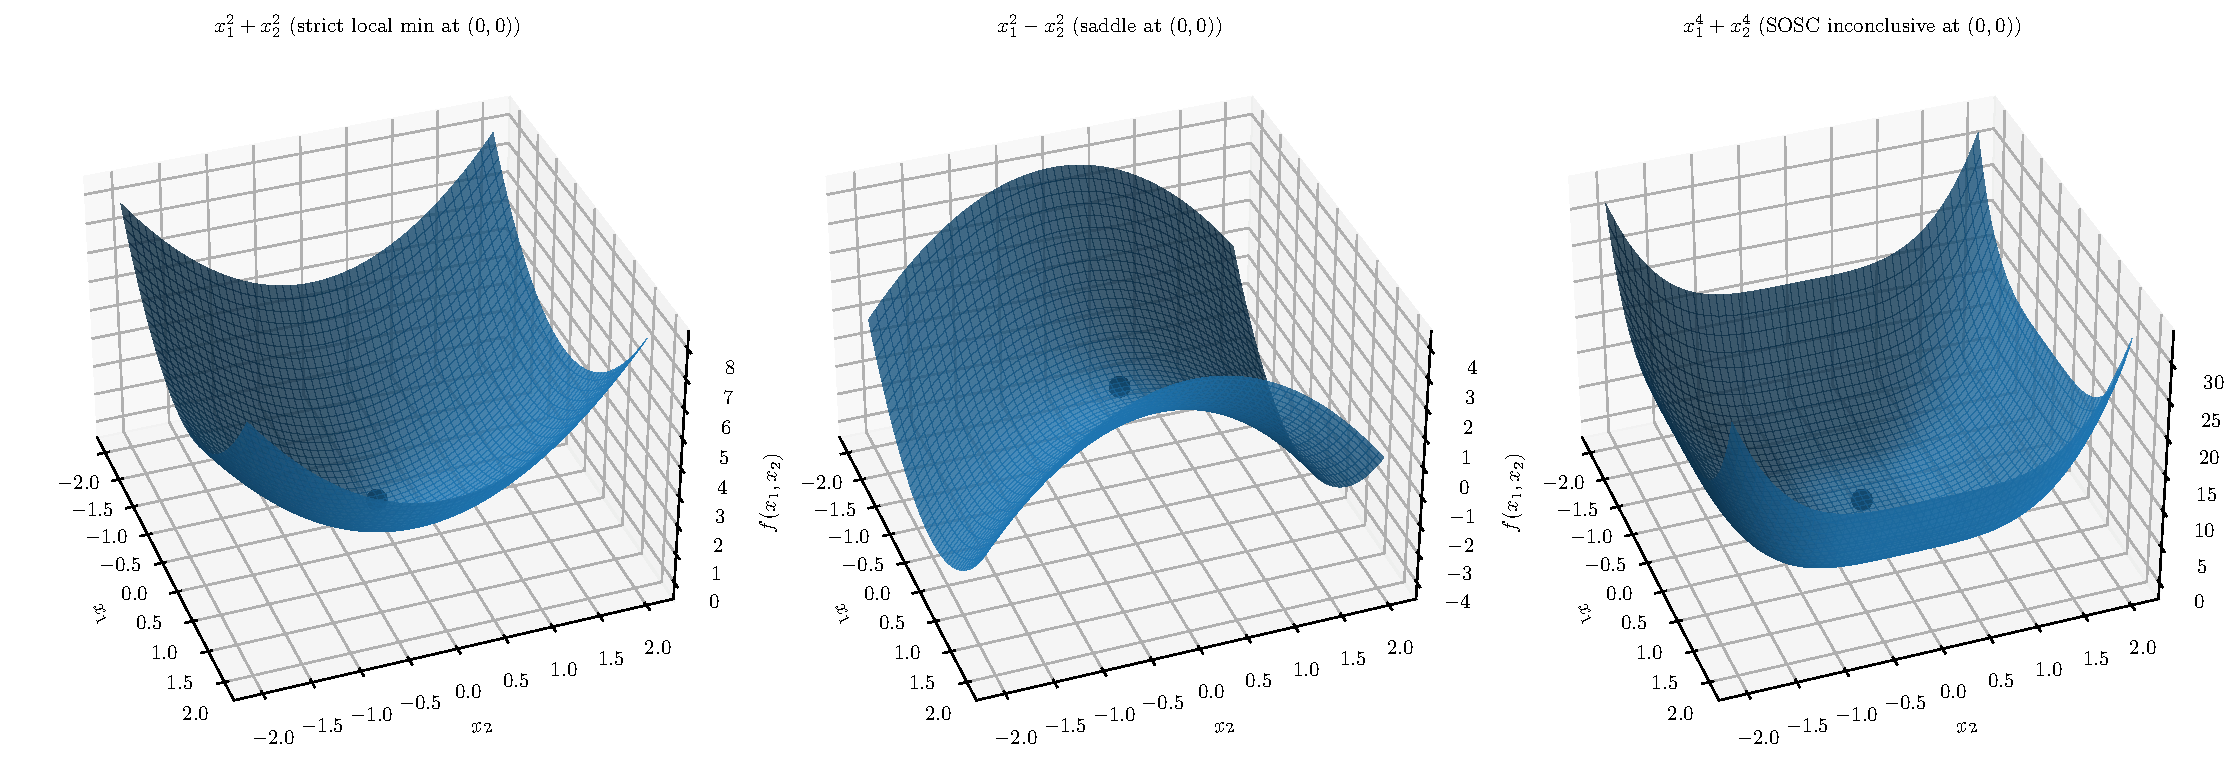
\includegraphics[width=0.8\textwidth]{figs/optimization/critical_points.pdf}
        \caption{The three functions from the example with the critical points labeled (black).}
        \label{fig:optimality-conditions}
    \end{figure}
    \end{exampleBox}


\begin{warningBox}
    \textbf{Warning}: A stationary point (where $\nabla f(\mathbf{x}^*) = 0$) is not necessarily a minimum. It could be a maximum or a saddle point. The second-order conditions using the Hessian are needed to distinguish between these cases. Optimization algorithms may converge to any stationary point, so verifying the nature of the solution is essential.
\end{warningBox}

\subsection{Proofs for Optimality Conditions}
We now provide proofs for the optimality conditions. Don't worry too much about the proofs if you find them difficult to parse---they are really just here for completeness, hence the asterisks on the section titles---but definitely make sure you understand the intuition behind them (\Cref{sec:optimality-conditions-intuition}).

Throughout, we assume that $f:\mathbb{R}^N\to\mathbb{R}$ is twice continuously differentiable in a neighborhood of $\mathbf{x}^*$. We repeatedly use the second-order Taylor expansion with remainder:
\begin{equation}\label{eq:taylor}
f(\mathbf{x}^* + \epsilon \mathbf{d})
= f(\mathbf{x}^*) 
  + \epsilon \nabla f(\mathbf{x}^*)^\top \mathbf{d}
  + \frac{1}{2}\epsilon^2 \mathbf{d}^\top \nabla^2 f(\mathbf{x}^*) \mathbf{d}
  + r(\epsilon,\mathbf{d})
\end{equation}
where the condition on the remainder $r(\epsilon,\mathbf{d})$ is that for every $\eta>0$ there exists $\bar{\epsilon}>0$ such that 
$\bigl|r(\epsilon,\mathbf{d})\bigr|\le \eta \epsilon^2$ whenever $0<\epsilon\le \bar{\epsilon}$ and $\|\mathbf{d}\|_2=1$.

\subsubsection{\texorpdfstring{First-Order Necessity (FONC)\textsuperscript{*}}{First-Order Necessity (FONC)}}
\emph{Claim.} If $\mathbf{x}^*$ is a local minimizer of $f$, then $\nabla f(\mathbf{x}^*)=\mathbf{0}$.

\emph{Proof.}
Assume by contradiction that $\nabla f(\mathbf{x}^*)\neq \mathbf{0}$. Let $\mathbf{d} := -\nabla f(\mathbf{x}^*)/\|\nabla f(\mathbf{x}^*)\|_2$ (the negative gradient direction). Then $\nabla f(\mathbf{x}^*)^\top \mathbf{d} = -\|\nabla f(\mathbf{x}^*)\|_2 < 0$. Using \autoref{eq:taylor} and the bound on the remainder,
\begin{equation}
f(\mathbf{x}^* + \epsilon \mathbf{d})
= f(\mathbf{x}^*) + \epsilon \nabla f(\mathbf{x}^*)^\top \mathbf{d} 
  + \frac{1}{2}\epsilon^2 \mathbf{d}^\top \nabla^2 f(\mathbf{x}^*) \mathbf{d} + r(\epsilon,\mathbf{d})
\end{equation}
For sufficiently small $\epsilon>0$, the negative linear term $\epsilon \nabla f(\mathbf{x}^*)^\top \mathbf{d}$ dominates the $O(\epsilon^2)$ terms, hence
$f(\mathbf{x}^*+\epsilon \mathbf{d}) < f(\mathbf{x}^*)$, contradicting local minimality. Therefore, $\nabla f(\mathbf{x}^*)=\mathbf{0}$.

\subsubsection{\texorpdfstring{Second-Order Necessity (SONC)\textsuperscript{*}}{Second-Order Necessity (SONC)}}
\emph{Claim.} If $\mathbf{x}^*$ is a local minimizer of $f$, then $\nabla^2 f(\mathbf{x}^*) \succeq \mathbf{0}$.

\emph{Proof.}
By the FONC just established, $\nabla f(\mathbf{x}^*)=\mathbf{0}$. Thus, the linear term in \autoref{eq:taylor} vanishes and we have, for any unit direction $\mathbf{d}$,
\begin{equation}
f(\mathbf{x}^* + \epsilon \mathbf{d})
= f(\mathbf{x}^*) + \frac{1}{2}\epsilon^2 \mathbf{d}^\top \nabla^2 f(\mathbf{x}^*) \mathbf{d} + r(\epsilon,\mathbf{d})
\end{equation}
Suppose, toward a contradiction, that $\nabla^2 f(\mathbf{x}^*) \nsucceq \mathbf{0}$. Then there exists $\mathbf{d}$ with $\|\mathbf{d}\|_2=1$ such that 
$\mathbf{d}^\top \nabla^2 f(\mathbf{x}^*) \mathbf{d} < 0$ (e.g., an eigenvector corresponding to a negative eigenvalue). Choosing $\epsilon>0$ small enough so that
\begin{equation}
|r(\epsilon,\mathbf{d})|\le \frac{1}{4}\epsilon^2  \left|\mathbf{d}^\top \nabla^2 f(\mathbf{x}^*) \mathbf{d}\right|
\end{equation} 
we obtain
\begin{equation}
f(\mathbf{x}^* + \epsilon \mathbf{d}) 
\le f(\mathbf{x}^*) + \frac{1}{2}\epsilon^2 \mathbf{d}^\top \nabla^2 f(\mathbf{x}^*) \mathbf{d} 
+ \frac{1}{4}\epsilon^2 \left|\mathbf{d}^\top \nabla^2 f(\mathbf{x}^*) \mathbf{d}\right|
< f(\mathbf{x}^*)
\end{equation}
contradicting local minimality. Hence, $\nabla^2 f(\mathbf{x}^*) \succeq \mathbf{0}$.

\subsubsection{\texorpdfstring{Second-Order Sufficiency (SOSC)\textsuperscript{*}}{Second-Order Sufficiency (SOSC)}}
\emph{Claim.} If $\nabla f(\mathbf{x}^*)=\mathbf{0}$ and $\nabla^2 f(\mathbf{x}^*) \succ \mathbf{0}$, then $\mathbf{x}^*$ is a \emph{strict} local minimizer.

\emph{Proof.}
Let $\mathbf{H}^* := \nabla^2 f(\mathbf{x}^*) \succ \mathbf{0}$ with smallest eigenvalue $\lambda_{\min}(\mathbf{H}^*)>0$, so
\begin{equation}
    \mathbf{d}^\top \mathbf{H}^* \mathbf{d} \ge \lambda_{\min}(\mathbf{H}^*)\, \|\mathbf{d}\|_2^2 \quad \text{for all }\mathbf{d}\in\mathbb{R}^N
    \label{eq:pd-bound}
\end{equation}
Using \autoref{eq:taylor} with $\nabla f(\mathbf{x}^*)=\mathbf{0}$, for any unit direction $\mathbf{d}$ and $\epsilon>0$,
\begin{equation}
f(\mathbf{x}^* + \epsilon \mathbf{d})
= f(\mathbf{x}^*) + \frac{1}{2}\epsilon^2 \mathbf{d}^\top \mathbf{H}^* \mathbf{d} + r(\epsilon,\mathbf{d}).
\end{equation}
We fix $\eta \in \bigl(0, \tfrac{1}{2}\lambda_{\min}(\mathbf{H}^*)\bigr)$. By the stated remainder bound, there exists $\bar{\epsilon}>0$ such that $|r(\epsilon,\mathbf{d})|\le \eta \epsilon^2$ for all unit $\mathbf{d}$ whenever $0<\epsilon\le \bar{\epsilon}$. Hence, for all unit $\mathbf{d}$ and $0<\epsilon\le\bar{\epsilon}$,
\begin{equation}
f(\mathbf{x}^* + \epsilon \mathbf{d})
\ge f(\mathbf{x}^*) + \Bigl(\frac{1}{2}\lambda_{\min}(\mathbf{H}^*) - \eta\Bigr)\epsilon^2
> f(\mathbf{x}^*)
\end{equation}
To handle an arbitrary nonzero increment $\boldsymbol{\Delta}$ with $\|\boldsymbol{\Delta}\|_2 \le \bar{\epsilon}$, we can write $\boldsymbol{\Delta}=\epsilon \mathbf{d}$ with $\epsilon=\|\boldsymbol{\Delta}\|_2$ and $\mathbf{d}=\boldsymbol{\Delta}/\|\boldsymbol{\Delta}\|_2$ (so $\|\mathbf{d}\|_2=1$); the previous inequality applies and gives $f(\mathbf{x}^*+\boldsymbol{\Delta})>f(\mathbf{x}^*)$. Thus, $\mathbf{x}^*$ is a strict local minimizer.


\subsubsection{Intuition}
\label{sec:optimality-conditions-intuition}
The proofs above formalize the intuition behind the optimality conditions:
\begin{itemize}
\item If $\nabla f(\mathbf{x}^*)\neq 0$, a small step in the negative gradient direction strictly decreases the objective (first-order term dominates), contradicting local minimality.
\item If $\nabla f(\mathbf{x}^*)=\mathbf{0}$ but $\nabla^2 f(\mathbf{x}^*)\nsucceq \mathbf{0}$, 
there exists a direction with negative curvature. Along that direction, the second-order term is negative and again decreases the objective.
\item If $\nabla f(\mathbf{x}^*)=\mathbf{0}$ and $\nabla^2 f(\mathbf{x}^*)\succ \mathbf{0}$, 
then the quadratic term is positive in every direction and dominates the remainder term, so nearby points have strictly larger objective value.
\end{itemize}

\section{Iterative Descent Methods}
Most numerical methods for unconstrained optimization are iterative. They start from an initial guess, $x_0$, and generate a sequence of points $\{x_k\}$ that converge to a local minimum. Indeed, we saw this before when we discussed fixed-point iterations for solving systems of linear equations (Jacobi and Gauss-Seidel iterations) and root-finding (Newton's method). The general form of such an iteration is
\begin{equation}
    \mathbf{x}_{k+1} = \mathbf{x}_k + \alpha_k \mathbf{d}_k
    \label{eq:iterative_update}
\end{equation}
where $\mathbf{d}_k$ is the \textbf{search direction} and $\alpha_k > 0$ is the \textbf{step size} (or step length). The primary difference between the methods discussed below lies in how they choose the search direction $\mathbf{d}_k$.

\subsection{Steepest Descent}
\label{sec:steepest-descent}
The \textbf{steepest descent} method, also called gradient descent and a first-order method, uses the most intuitive search direction: the one in which the objective function $f(\mathbf{x})$ decreases most rapidly. We consider a first-order Taylor expansion of $f(\mathbf{x})$ around $\mathbf{x}_k$:
\begin{equation}
f(\mathbf{x}_k+\alpha_k\mathbf{d}_k)\approx f(\mathbf{x}_k) + \alpha_k \nabla f(\mathbf{x}_k)^{\top}\mathbf{d}_k
\end{equation}
For a fixed $\alpha_k>0$, the linear term determines whether we go up or down. We decrease $f$ as fast as possible by pointing $\mathbf{d}_k$ directly opposite the gradient because, among all unit directions, this minimizes $\nabla f(\mathbf{x}_k)^{\top}\mathbf{d}_k$. This gives the steepest-descent direction
\begin{equation}
\mathbf{d}_k=-\nabla f(\mathbf{x}_k), \qquad
\mathbf{x}_{k+1}=\mathbf{x}_k-\alpha_k\nabla f(\mathbf{x}_k)
\end{equation}
The step size $\alpha_k$ plays a very important role here. If the step is tiny, we faithfully follow the gradient but creep along level sets, so progress is slow, and the path looks like short arrows tangent to the valley walls (perpendicular to the level sets) as we inch toward the center. If the step is too large, we overshoot the valley, bounce across contours, and the iterates can zig-zag or even blow up. We show this in \autoref{fig:steepest-descent}.

\begin{figure}[H]
    \centering
    \begin{tikzpicture}[line cap=round,line join=round,>=Stealth, scale=0.5]

        %---------------------------------------
        % helper: a stack of slanted ellipses
        %---------------------------------------
        \def\ellipses{
            \foreach \s in {1.00,1.45,1.90,2.35,2.80}{
                \draw[thick] (0,0) ellipse [
                    x radius={2.0cm*\s},
                    y radius={0.9cm*\s},
                    rotate=10
                ];
            }
        }

        %====================
        % LEFT: small step size
        %====================
        \begin{scope}
            % title
            \node[font=\large] at (0,3.6) {small step size};

            % concentric level sets
            \ellipses

            % minimizer point
            \node[star,star points=5,star point ratio=2.25,minimum size=6pt,fill=red,scale=0.5] at (0,0) {};

            % start marker
            \coordinate (Ls) at (4.7,2.0);
            \fill (Ls) circle (4pt);
            \node[above=4pt] at (Ls) {$x_0$};

            % descent path (small steps, moving inward)
            \coordinate (L0) at (4.45,1.35);
            \coordinate (L1) at (3.75,1.05);
            \coordinate (L2) at (3.05,0.75);
            \coordinate (L3) at (2.30,0.48);
            \coordinate (L4) at (1.60,0.25);
            \coordinate (L5) at (0.95,0.10);
            \coordinate (L6) at (0.25,0.02);

            % short first move from star
            \draw[thick,->] (Ls) -- (L0);

            % step-by-step arrows inward
            \foreach \k/\n in {0/1,1/2,2/3,3/4,4/5,5/6}{
                \draw[-{Stealth[length=3mm,width=2mm]},thick] (L\k) -- (L\n);
            }
        \end{scope}

        %====================
        % RIGHT: too large step size
        %====================
        \begin{scope}[xshift=12.4cm]
            % title
            \node[font=\large] at (0,3.6) {too large step size};

            % concentric level sets
            \ellipses

            % minimizer point
            \node[star,star points=5,star point ratio=2.25,minimum size=6pt,fill=red,scale=0.5] at (0,0) {};

            % start marker
            \coordinate (Rs) at (4.7,2.0);
            \fill (Rs) circle (4pt);
            \node[above=4pt] at (Rs) {$x_0$};

            % descent path (overshooting, zig-zagging)
            \coordinate (R0) at (4.45,1.35);
            \coordinate (R1) at (3.15,-0.95);
            \coordinate (R2) at (2.25,1.20);
            \coordinate (R3) at (1.30,-0.85);
            \coordinate (R4) at (0.55,1.05);
            \coordinate (R5) at (-0.10,-0.70);

            % short first move from star
            \draw[thick,->] (Rs) -- (R0);

            % big, oscillatory steps
            \foreach \k/\n in {0/1,1/2,2/3,3/4,4/5}{
                \draw[-{Stealth[length=3mm,width=2mm]},thick] (R\k) -- (R\n);
            }
        \end{scope}

    \end{tikzpicture}
    \caption{Steepest descent method. Left: small step size; right: too large step size.}
    \label{fig:steepest-descent}
\end{figure}

\subsubsection{Backtracking Line Search}
How, then, should we pick $\alpha_k$ in practice? One way is via a backtracking line search. Start with a trial step (often $\alpha_k=1$ or a value carried over from the previous iteration) and check whether the new point actually reduces the objective by a reasonable amount. A convenient ``sufficient decrease'' test is the Armijo condition with constant $1/2$:
\begin{equation}
f\!\left(\mathbf{x}_k-\alpha_k\nabla f(\mathbf{x}_k)\right)\le
f(\mathbf{x}_k)-\frac{1}{2}\alpha_k\|\nabla f(\mathbf{x}_k)\|_2^2
\end{equation}
If this inequality holds, we accept the step and move on. If it fails, we shrink the step (e.g., halve it) and try again. This simple loop tends to accept larger steps when the local model is reliable and automatically backs off when the function is curved or the first-order approximation is poor.

It is sometimes helpful to start backtracking with an educated guess for the step length. A second-order Taylor model around $\mathbf{x}_k$ gives
\begin{equation}
f(\mathbf{x}_k-\alpha_k\nabla f(\mathbf{x}_k))
\approx
f(\mathbf{x}_k)
-\alpha_k \nabla f(\mathbf{x}_k)^{\top}\nabla f(\mathbf{x}_k)
+\frac{1}{2}\alpha_k^{2} \nabla f(\mathbf{x}_k)^{\top}\nabla^2 f(\mathbf{x}_k)\,\nabla f(\mathbf{x}_k)
\end{equation}
Minimizing this quadratic in $\alpha_k$ yields
\begin{equation}
\alpha_k^\ast
=
\frac{\nabla f(\mathbf{x}_k)^{\top}\nabla f(\mathbf{x}_k)}{\nabla f(\mathbf{x}_k)^{\top}\nabla^2 f(\mathbf{x}_k)\nabla f(\mathbf{x}_k)}
\end{equation}
Using $\alpha_k^\ast$ as the initial guess often reduces the number of backtracking trials, although it requires access to second derivatives (or at least Hessian-vector products), which may be expensive or unavailable.

\begin{exampleBox}
\textbf{Example: Backtracking line search.}
    The use of backtracking line search becomes especially clear when we consider a function such as
    \[
    f(\mathbf{x}) = x_1^2 + 10x_2^2
    \]
    whose level sets are elongated ellipses. Pure steepest descent alternates between moving mostly in the $x_1$ direction and then mostly in $x_2$, producing a characteristic zig-zag down the valley. Small steps make the zig-zag gentle but slow; large steps leap across the valley and risk divergence; backtracking threads the needle by taking steps that are as large as the local geometry allows (see Figure~\ref{fig:anisotropic}).

    \begin{figure}[H]
        \centering
        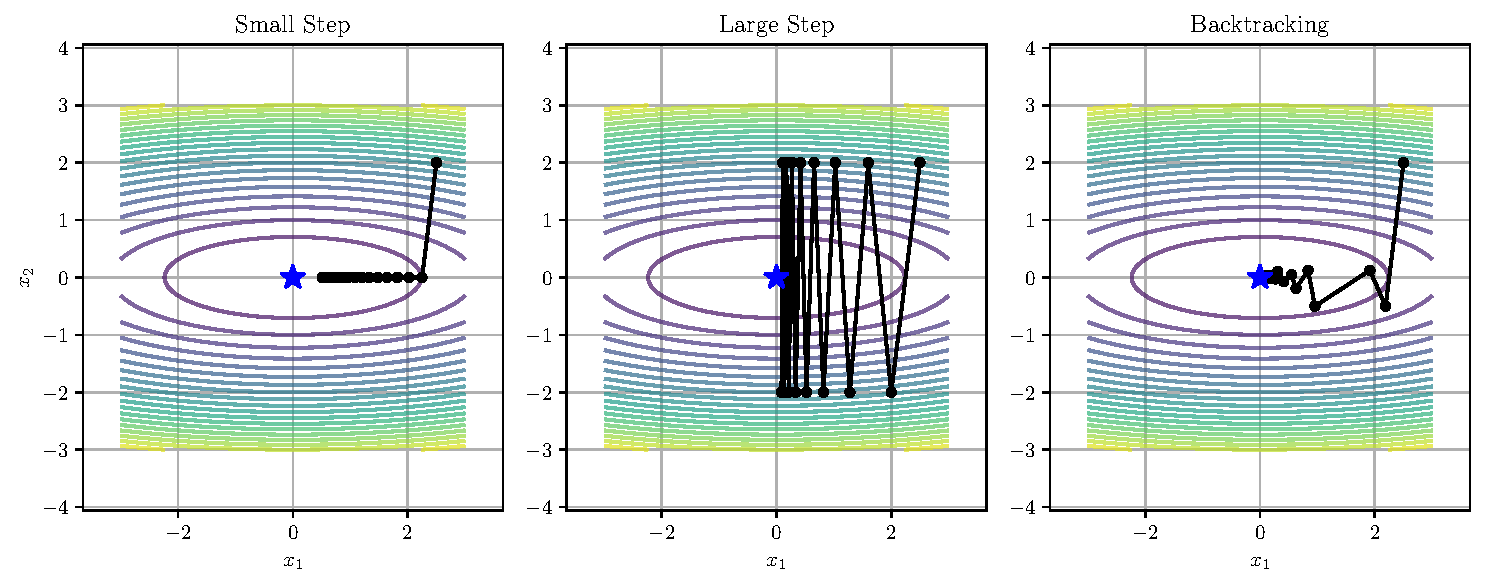
\includegraphics[width=.98\textwidth]{figs/optimization/backtracking_example.pdf}
        \caption{Gradient descent trajectories on $f(x_1,x_2)=x_1^2+10x_2^2$: 
        small step size (left), too large step size (middle), and backtracking (right). The blue star is the global minimum.}
        \label{fig:anisotropic}
    \end{figure}

\end{exampleBox}

\subsubsection{Convergence} From a theoretical standpoint, under mild smoothness assumptions and with a proper line search, the gradient norms go to zero:
\begin{equation}
\lim_{k\to\infty}\|\nabla f(\mathbf{x}_k)\|_p=0
\end{equation}
so every limit point is stationary. This property is also known as global convergence. When the iterates enter a neighborhood of a nondegenerate minimizer, the method converges linearly:
\begin{equation}
\frac{f(\mathbf{x}_{k+1})-f(\mathbf{x}^\ast)}{f(\mathbf{x}_k)-f(\mathbf{x}^\ast)}\le r
\quad\text{for some } r\in(0,1)
\end{equation}
The constant $r$ is governed by the condition number of the Hessian near $\mathbf{x}^\ast$. Poor conditioning (long, narrow valleys) slows the rate and accentuates the zig-zag, which is why steepest descent can require many iterations on ill-conditioned problems.

\subsubsection{Stochastic Gradient Descent} 
Modern large-scale problems introduce another complication: evaluating the full gradient can be the dominant cost. If the objective is a sum of many data-dependent losses, $\min_{\mathbf{x}}\sum_{k=1}^{N} f_k(\mathbf{x}),$ computing $\nabla \sum_k f_k$ each iteration may be prohibitive. Stochastic gradient descent replaces the full sum with a randomly selected data term or a small mini-batch, producing the update $\mathbf{x}_{k+1}=\mathbf{x}_k-\alpha_k \nabla f_{i_k}(\mathbf{x}_k)$. The price is additional noise, and the benefit is dramatically cheaper steps and faster progress per unit time on huge datasets. Learning-rate schedules and variance-reduction tricks are then used to recover stable convergence.

All of this explains why steepest descent is so common and powerful while still having some (sometimes major) drawbacks. It is conceptually simple and easy to implement---just compute a gradient, pick a step length, and move downhill---and it requires only first-order information. Yet, the convergence is merely linear and can be painfully slow on ill-conditioned landscapes, and even computing the gradient may be costly at scale. These drawbacks motivate practical enhancements (line search, preconditioning, momentum, quasi-Newton methods) and sampling strategies (SGD and its variants) that preserve the core idea (follow the direction of fastest local decrease) while coping better with curvature and data size.

\subsection{Newton and Modified-Newton Methods}
\label{sec:newton}
In steepest descent, we search for a minimum by moving in the direction of greatest decrease. Newton's method takes a different perspective: instead of searching, it directly tries to solve the optimality condition
\begin{equation}
\nabla f(\mathbf{x}) = \mathbf{0}
\end{equation}
which characterizes stationary points of $f$. Notice the similarity with a general nonlinear system of equations. Earlier, we solved problems of the form
\begin{equation}
\mathbf{g}(\mathbf{x}) = \mathbf{0}, \qquad \mathbf{g}:\mathbb{R}^N \to \mathbb{R}^N
\end{equation}
using Newton's method. Optimization fits this framework if we set
\begin{equation}
\mathbf{g}(\mathbf{x}) := \nabla f(\mathbf{x})
\end{equation}
Thus, finding a stationary point of $f$ is equivalent to solving a system of nonlinear equations (solving for the roots of $\mathbf{g}(\mathbf{x})$). The Jacobian of $\mathbf{g}(\mathbf{x})$ is
\begin{equation}
\mathbf{J}_g(\mathbf{x}) = \nabla(\nabla f(\mathbf{x})) = \nabla^2 f(\mathbf{x})
\end{equation}
which is precisely the Hessian of $f$. Therefore, Newton's method for optimization naturally uses the Hessian. A Newton update step takes the form
\begin{equation}
\mathbf{x}_{k+1} = \mathbf{x}_k + \alpha_k \mathbf{d}_k,
\qquad
\mathbf{d}_k = -\left(\nabla^2 f(\mathbf{x}_k)\right)^{-1}\nabla f(\mathbf{x}_k)
\label{eq:newton_direction}
\end{equation}
where $\alpha_k > 0$ is the step length (often chosen by line search). So we can see that Newton's method for optimization is nothing more than Newton's method for nonlinear equations, specialized to the gradient system $\nabla f(\mathbf{x})=0$, with the Hessian playing the role of the Jacobian.

To understand why this works, recall that near a point $\mathbf{x}_k$, the function $f$ can be locally approximated by its second-order Taylor expansion:
\begin{equation}
f(\mathbf{x}) \approx f(\mathbf{x}_k) 
+ \nabla f(\mathbf{x}_k)^\top(\mathbf{x}-\mathbf{x}_k) 
+ \frac{1}{2}(\mathbf{x}-\mathbf{x}_k)^\top \nabla^2 f(\mathbf{x}_k)(\mathbf{x}-\mathbf{x}_k)
\end{equation}
This quadratic model has a stationary point where its gradient vanishes. Solving for that point gives exactly the Newton step direction $\mathbf{d}_k$. Notice that we are using curvature information to find the step direction in contrast to only the first-order information being used in steepest descent.

\textbf{Choosing the step length.}\quad
Close to a minimizer and under mild smoothness, taking a full step $\alpha_k=1$ is appropriate and yields rapid local convergence. Farther away, a line search is employed for best performance in exactly the same way as in steepest descent.

\subsubsection{Hessian Modification}
Solving the stationarity equation $\nabla f(\mathbf{x})=\mathbf{0}$ does not by itself distinguish minima from saddles or maxima. Consequently, the plain Newton step $\mathbf{d}_k$ in \eqref{eq:newton_direction} can fail to decrease $f$ when the Hessian $\nabla^2 f(\mathbf{x}_k)$ is indefinite or singular.

A simple way to see what we need is to examine the predicted change in $f$ from a Newton step. Using the quadratic model of $f$ at $\mathbf{x}_k$ and substituting $\mathbf{d}_k=-\big(\nabla^2 f(\mathbf{x}_k)\big)^{-1}\nabla f(\mathbf{x}_k)$, we obtain the model-predicted decrease
\begin{equation}
f(\mathbf{x}_{k+1})-f(\mathbf{x}_k)
\approx
-\nabla f(\mathbf{x}_k)^\top
\big(\nabla^2 f(\mathbf{x}_k)\big)^{-1}
\nabla f(\mathbf{x}_k)
\end{equation}
For the right-hand side to be negative for every nonzero gradient, we must have
\begin{equation}
\big(\nabla^2 f(\mathbf{x}_k)\big)^{-1} \succ 0 
\quad\iff\quad 
\nabla^2 f(\mathbf{x}_k)\succ 0
\end{equation}
i.e., the Hessian must be positive definite (PD). If the Hessian is not PD, Newton's direction is not guaranteed to be a descent direction.

So what does this tell us? We want a PD Hessian. Luckily, we can modify the Hessian to make it PD whenever necessary. The simplest and very effective modification is a diagonal shift:
\begin{equation}
\mathbf{d}_k(\delta_k)
=
-\big(\nabla^2 f(\mathbf{x}_k)+\delta_k \mathbf{I}\big)^{-1}\nabla f(\mathbf{x}_k),
\qquad \delta_k\ge 0
\end{equation}
followed by a (backtracking) line search to pick $\alpha_k>0$, and then
\begin{equation}
\mathbf{x}_{k+1}=\mathbf{x}_k+\alpha_k\mathbf{d}_k(\delta_k).
\end{equation}
As soon as $\nabla^2 f(\mathbf{x}_k)+\delta_k\mathbf{I}\succ 0$, the direction is guaranteed to be a descent direction because
\begin{equation}
\nabla f(\mathbf{x}_k)^\top \mathbf{d}_k(\delta_k)
=
-\nabla f(\mathbf{x}_k)^\top
\big(\nabla^2 f(\mathbf{x}_k)+\delta_k \mathbf{I}\big)^{-1}
\nabla f(\mathbf{x}_k)
<0
\quad\text{whenever}\quad \nabla f(\mathbf{x}_k)\ne \mathbf{0}
\end{equation}
The line search then ensures an actual decrease in the objective. When choosing $\delta_k$, we want to keep Newton's fast local behavior, so we aim for a small positive shift.

\subsubsection{Global and Local Convergence}
With standard line-search safeguards (e.g., sufficient decrease), Newton and modified-Newton iterations produce a sequence for which the gradient norms tend to zero, i.e., global convergence to a stationary point. Once the iterates enter a neighborhood of a nondegenerate minimizer $\mathbf{x}^\ast$ with positive-definite Hessian, the pure Newton method (i.e., $\alpha_k=1$, no modification to the Hessian) is \emph{quadratically convergent}:
\begin{equation}
\lim_{k\to\infty}\frac{\|\mathbf{x}_{k+1}-\mathbf{x}^\ast\|}{\|\mathbf{x}_k-\mathbf{x}^\ast\|^2}=C,\qquad C>0
\label{eq:newton_quadratic_convergence}
\end{equation}
This is faster than the linear convergence characteristic of steepest descent and explains Newton's dramatic acceleration in practice as the solution is approached.  

\textbf{R-convergence.}\quad
Let $e_k:=\|\mathbf{x}_k-\mathbf{x}^\ast\|$. The limit \autoref{eq:newton_quadratic_convergence} (known as Q-convergence) is a stepwise statement about the actual errors: for any $\varepsilon\in(0,1)$ there exists $K$ such that
\begin{equation}
e_{k+1}\le (C+\varepsilon)e_k^{2}\qquad(k\ge K)
\end{equation}
R-convergence instead bounds these (possibly wiggly) errors by a smooth envelope. We say $\{\mathbf{x}_k\}$ R-converges to $\mathbf{x}^\ast$ with order $p\ge 1$ if there exist $K\in\mathbb{N}$, $C'>0$, and a sequence $\{v_k\}$ with $v_k\to 0$ such that for all $k\ge K$,
\begin{equation}
e_k\le v_k,\qquad v_{k+1}\le C' v_k^{p}
\end{equation}
Special cases are $p=1$ (R-linear), $p>1$ (R-superlinear), and $p=2$ (R-quadratic).

We can use \autoref{eq:newton_quadratic_convergence} to show that Newton has local R-quadratic convergence, i.e., capturing quadratic overall decay even if individual steps fluctuate (e.g., due to line search or noise). We fix $\varepsilon\in(0,1)$ and $K$ as above. We set $v_K:=e_K$ and define $v_{k+1}:=(C+\varepsilon) v_k^{2}$. Then $e_k\le v_k$ for all $k\ge K$ and $v_{k+1}\le (C+\varepsilon)v_k^{2}$, so Newton has local R-quadratic convergence.

R-convergence is weaker than the stepwise Q-quadratic statement in \autoref{eq:newton_quadratic_convergence}: Q-quadratic $\implies$ R-quadratic, but not conversely. We care about R-convergence because line searches, Hessian modifications, or noise can make the actual errors oscillate. R-convergence still guarantees an overall quadratic decay by bounding the errors with a smooth envelope even when the per-iteration ratio does not stabilize.

% MC:
% TODO: add figure showing Q-convergence and R-convergence differences
% although, I'm not sure that 10.34 really necessitates a distinction between these two notions of convergence (?)

\subsubsection{Comparison with Steepest Descent}
Steepest descent takes steps along $-\nabla f(\mathbf{x}_k)$ and relies on a one-dimensional line search; Newton takes the $N$-dimensional quadratic-model minimizer $\mathbf{d}_k=-\nabla^2 f(\mathbf{x}_k)^{-1}\nabla f(\mathbf{x}_k)$. Consequently, Newton typically requires far fewer iterations and exhibits a much steeper drop in the objective near the optimum, at the price of assembling curvature information and solving a linear system each iteration.

% MC: I'd rather change this figure to actual Python code plots for believability purposes, but leaving this for now
\begin{figure}[H]
\centering
\begin{tikzpicture}[line cap=round,line join=round,>=Stealth, scale=0.55]
\def\ellipses{
\foreach \s in {1.0,1.45,1.9,2.35,2.8}{
\draw[thick] (0,0) ellipse [x radius={2.0cm*\s}, y radius={0.9cm*\s}, rotate=12];
}
}
% Left: steepest descent path
\begin{scope}
\node[font=\large] at (0,3.8) {steepest descent};
\ellipses
\node[star,star points=5,star point ratio=2.25,minimum size=6pt,fill=red,scale=0.5] at (0,0) {};
\coordinate (s0) at (4.6,2.1);
\fill (s0) circle (4pt);
\node[above=4pt] at (s0) {$x_0$};
\coordinate (s1) at (3.9,1.1);
\coordinate (s2) at (2.6,0.6);
\coordinate (s3) at (1.7,0.3);
\coordinate (s4) at (0.7,0.1);
\draw[thick,->] (s0)--(s1);
\foreach \a/\b in {1/2,2/3,3/4}{
\draw[-{Stealth[length=3mm,width=2mm]},thick] (s\a)--(s\b);
}
\end{scope}
% Right: Newton steps
\begin{scope}[xshift=12.6cm]
\node[font=\large] at (0,3.8) {Newton};
\ellipses
\node[star,star points=5,star point ratio=2.25,minimum size=6pt,fill=red,scale=0.5] at (0,0) {};
\coordinate (n0) at (4.6,2.1);
\fill (n0) circle (4pt);
\node[above=4pt] at (n0) {$x_0$};
\coordinate (n1) at (1.4,0.2);
\coordinate (n2) at (0.02,0.01);
\draw[thick,->] (n0)--(n1);
\draw[-{Stealth[length=3mm,width=2mm]},thick] (n1)--(n2);
\end{scope}
\end{tikzpicture}
\caption{Steepest descent “searches” along the gradient direction, while Newton “solves” a local quadratic model and often reaches the minimizer in far fewer steps on well-conditioned problems.}
\label{fig:sd-vs-newton}
\end{figure}

% \begin{exampleBox}
% \textbf{Example: Newton versus steepest descent.}
% TODO: add example that clearly shows where Newton is better than steepest descent due to curvature info
% \end{exampleBox}

\subsection{Quasi-Newton Methods}
Newton's method converges quickly (assuming the Hessian is positive definite and we are ``close enough'' to the solution initially), but each step depends on the exact Hessian $\nabla^{2} f(\mathbf{x}_k)$ and on solving a linear system with that matrix. For problems of dimension $N$, forming and storing the Hessian already costs on the order of $O(N^{2})$, and solving a dense linear system costs about $O(N^{3})$. On large problems, these costs make a Newton step impractical. This motivates \textbf{quasi-Newton methods}. These methods reuse information gathered along the iterations to build a good approximation to curvature---either to the Hessian itself or to its inverse---while using only gradient evaluations.\footnote{It's worth keeping in mind that we (almost always) do not explicitly invert a matrix in practice. When we ``use the inverse,'' we mean that we apply an approximation that plays the role of $[\nabla^2 f(\mathbf{x}_k)]^{-1}$.}

To connect this idea with Newton's method and make it more concrete, recall the Newton direction $\mathbf{d}_k$ obtained from
\begin{equation}
\nabla^{2} f(\mathbf{x}_k) \mathbf{d}_k = -\nabla f(\mathbf{x}_k)
\end{equation}
followed by a step $\mathbf{x}_{k+1} = \mathbf{x}_k + \alpha_k \mathbf{d}_k$ with a line search choosing $\alpha_k>0$. In a quasi-Newton method, we replace the exact Hessian by an \emph{approximate} Hessian $\mathbf{H}_k$ and compute the direction from
\begin{equation}
\mathbf{H}_k \mathbf{d}_k = -\nabla f(\mathbf{x}_k), \qquad \mathbf{x}_{k+1} = \mathbf{x}_k + \alpha_k \mathbf{d}_k
\end{equation}
Equivalently, one may make an approximation to the inverse Hessian and apply it to the gradient (using then $\mathbf{d}_k = -\mathbf{H}_k^{-1} \nabla f(\mathbf{x}_k)$); both views are common. The key question is how to update $\mathbf{H}_k$ as we learn more about the function. Taylor's theorem suggests that over a single step the gradient changes approximately linearly with displacement:
\begin{equation}
\nabla f(\mathbf{x}_{k+1}) - \nabla f(\mathbf{x}_k) \approx \nabla^{2} f(\mathbf{x}_{k+1}) (\mathbf{x}_{k+1}-\mathbf{x}_k)
\end{equation}
Quasi-Newton updates enforce this relationship exactly for the model we are building, leading to the \textbf{secant equation}
\begin{equation}
    \nabla f(\mathbf{x}_{k+1}) - \nabla f(\mathbf{x}_k) = \mathbf{H}_{k+1} (\mathbf{x}_{k+1}-\mathbf{x}_k)
    \label{eq:secant_equation}
\end{equation}


\subsubsection{Broyden-Fletcher-Goldfarb-Shanno (BFGS) Update}
We introduce the notation
\begin{equation}
\Delta\mathbf{x}_k := \mathbf{x}_{k+1}-\mathbf{x}_k,
\qquad
\Delta\mathbf{g}_k := \nabla f(\mathbf{x}_{k+1})-\nabla f(\mathbf{x}_k)
\end{equation}
so the constraint \autoref{eq:secant_equation} becomes 
\begin{equation}
    \mathbf{H}_{k+1}\Delta\mathbf{x}_k=\Delta\mathbf{g}_k
    \label{eq:bfgs_secant_equation}
\end{equation}
Among all matrices that satisfy this linear relation, we want an update that (1) keeps \(\mathbf{H}_{k+1}\) close to \(\mathbf{H}_k\), and (2) preserves positive definiteness so that the search direction remains a descent direction. Imposing these requirements leads to the \textbf{BFGS} formula in Hessian form:
\begin{equation}
    \mathbf{H}_{k+1}
    = \mathbf{H}_k
    + \frac{\Delta\mathbf{g}_k\Delta\mathbf{g}_k^{\!\top}}{\Delta\mathbf{g}_k^{\!\top}\Delta\mathbf{x}_k}
    - \frac{\mathbf{H}_k\Delta\mathbf{x}_k\Delta\mathbf{x}_k^{\!\top}\mathbf{H}_k^{\!\top}}
        {\Delta\mathbf{x}_k^{\!\top}\mathbf{H}_k\Delta\mathbf{x}_k}
    \label{eq:bfgs_hessian_form}
\end{equation}
By construction, the secant equation \autoref{eq:bfgs_secant_equation} holds exactly. Moreover, if \(\mathbf{H}_k\succ0\) and the line search enforces the curvature condition \(\Delta\mathbf{g}_k^{\!\top}\Delta\mathbf{x}_k>0\) (e.g., Wolfe conditions), then \(\mathbf{H}_{k+1}\succ0\) as well. Thus, no separate Hessian modification is required.

It is often convenient to apply the update directly to the inverse. Exploiting that the BFGS step is a rank-2 modification and using the Sherman-Morrison-Woodbury identity yields the inverse form
\begin{equation}
    \mathbf{H}_{k+1}^{-1}
    = \mathbf{H}_k^{-1}
    + \frac{(\Delta\mathbf{x}_k^{\!\top}\Delta\mathbf{g}_k)+\Delta\mathbf{g}_k^{\!\top}\mathbf{H}_k^{-1}\Delta\mathbf{g}_k}
        {(\Delta\mathbf{g}_k^{\!\top}\Delta\mathbf{x}_k)^2}\,
    \Delta\mathbf{x}_k\Delta\mathbf{x}_k^{\!\top}
    - \frac{\mathbf{H}_k^{-1}\Delta\mathbf{g}_k\,\Delta\mathbf{x}_k^{\!\top}
            + \Delta\mathbf{x}_k\,\Delta\mathbf{g}_k^{\!\top}\mathbf{H}_k^{-1}}
        {\Delta\mathbf{g}_k^{\!\top}\Delta\mathbf{x}_k}
    \label{eq:bfgs_inverse_form}
\end{equation}
which allows updating and applying \(\mathbf{H}_{k+1}^{-1}\) without solving a new linear system, thereby avoiding the \(O(N^3)\) cost of a dense factorization at each iteration.

With \(\mathbf{H}_k \approx \nabla^2 f(\mathbf{x}_k)\) (or \(\mathbf{H}_k^{-1} \approx [\nabla^2 f(\mathbf{x}_k)]^{-1}\)) available, the search direction is
\begin{equation}
\mathbf{d}_k = -\mathbf{H}_k^{-1}\nabla f(\mathbf{x}_k)
\end{equation}
and a line search selects \(\alpha_k>0\). The iterate is then updated by \(\mathbf{x}_{k+1}=\mathbf{x}_k+\alpha_k\mathbf{d}_k\). There is no universally optimal choice of the initial matrix \(\mathbf{H}_0\). We often start from a positive multiple of the identity, \(\mathbf{H}_0=\gamma\mathbf{I}\) with \(\gamma>0\).

\subsubsection{Convergence}
Under standard smoothness assumptions, BFGS with a proper line search enjoys the same global convergence guarantees as gradient descent (convergence to a stationary point). Locally, once \(\mathbf{x}_k\) is sufficiently close to a nondegenerate minimizer \(\mathbf{x}^\star\), the convergence is \emph{superlinear}:
\begin{equation}
\lim_{i\to\infty}
\frac{\|\mathbf{x}_{k+1}-\mathbf{x}^\star\|_p}{\|\mathbf{x}_k-\mathbf{x}^\star\|_p}=0.
\end{equation}
This means BFGS is typically faster than steepest descent and somewhat slower than exact Newton steps, which means it often gives an effective balance between per-iteration cost and speed of convergence. Because of this, it is the default algorithm used by \texttt{fminunc} in MATLAB.

% could mention limited-memory BFGS here


\begin{exampleBox}
    \textbf{Example: Adversarial Surfaces to Compare GD, BFGS, and Newton Methods.}
    We visualize how different update rules behave on three $2$D objectives specifically chosen to challenge the assumptions of each method. We take inspiration from the Wikipedia page on \href{https://en.wikipedia.org/wiki/Test_functions_for_optimization}{test functions for optimization}.
    
    All optimizers use a backtracking line search. We compare four algorithms: standard gradient descent (GD), BFGS (in inverse form with a curvature check), a robust modified Newton that shifts the Hessian to be positive definite using a small positive constant, and a standard, unmodified Newton's method. In the plots, a star marks the start point and an `x' marks the endpoint of each trajectory.
    
    \textbf{Case 1: A Sharp Crease.}
    Here, we use a smoothed absolute value function
    \begin{equation*}
        f(x,y) = \sqrt{x^2 + \epsilon} + \frac{1}{2}y^2
    \end{equation*}
    which has a sharp ``V''-shaped valley. This geometry directly violates the core assumption of Newton's method: that the function is well-approximated by a quadratic.

    \begin{figure}[H]
        \centering
        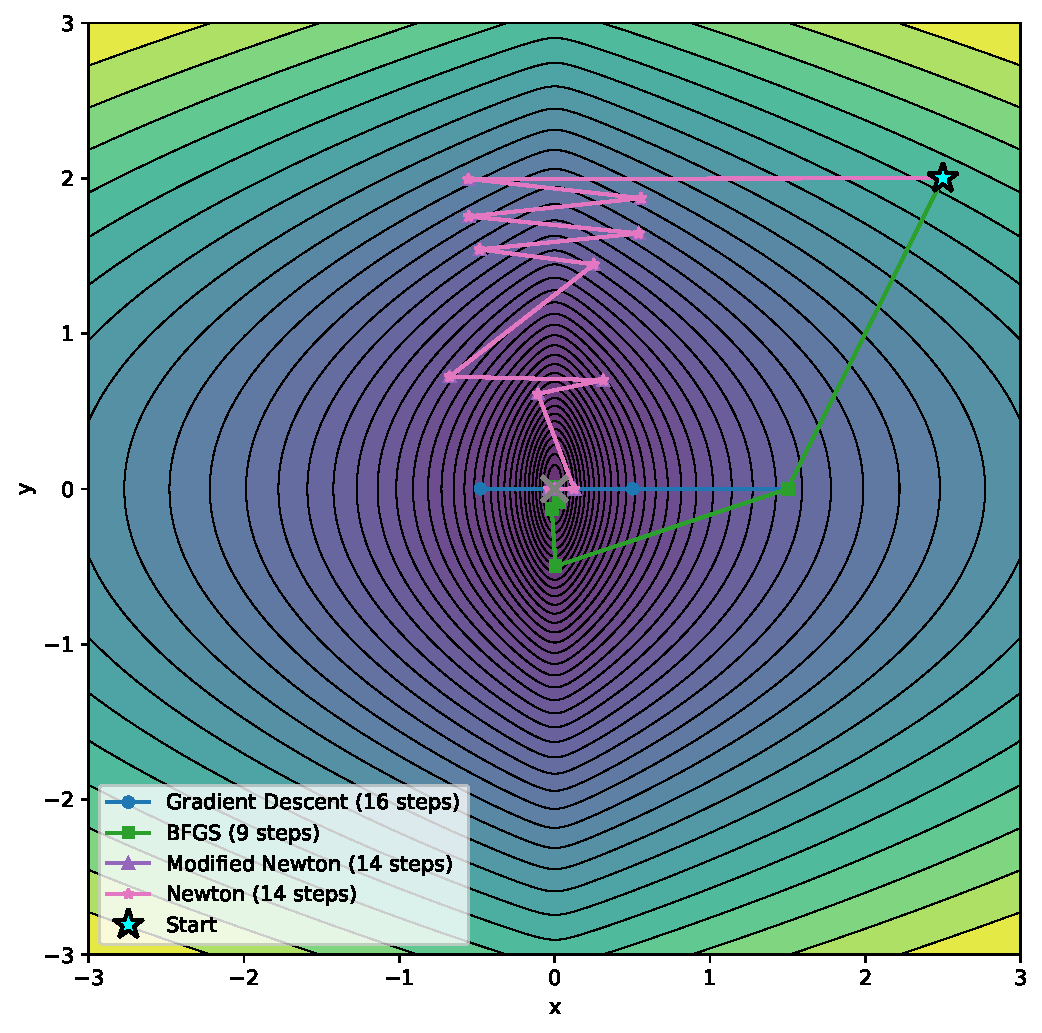
\includegraphics[width=.5\textwidth]{figs/optimization/paths_crease.pdf}
        \caption{Sharp Crease: Newton's method fails spectacularly due to a poor quadratic fit, while the more adaptive BFGS excels.}
    \end{figure}
    
    This scenario demonstrates a common failure mode for Newton's method. At the start point, the function is almost linear along the $x$-axis, so the Hessian is nearly zero. The resulting quadratic model is a terrible fit, causing Newton's method to overshoot the minimum and then oscillate back and forth. The line search prevents divergence, but the path is highly inefficient. On the other hand, BFGS is the clear winner. By building its curvature model gradually over several steps, it creates a more stable, averaged approximation that allows it to navigate the sharp turn smoothly and efficiently.
    
    % TODO: need to add more examples, or they can be saved for an exam!
\end{exampleBox}


\subsection{\texorpdfstring{Step Selection Paradigms\textsuperscript{*}}{Step Selection Paradigms}}
\label{sec:step-selection}
There are two standard ways to decide how far to move at each iterate and in which direction. They differ in the order of these choices.

\textbf{Line search.} We have always used this paradigm so far. First determine the step direction (e.g., steepest descent $-\nabla f(\mathbf{x}_k)$, Newton $-\big(\nabla^2 f(\mathbf{x}_k)\big)^{-1}\nabla f(\mathbf{x}_k)$, or a quasi-Newton direction), and then determine the step length $\alpha_k>0$ by searching along the ray
\begin{equation}
    \mathbf{x}_k+\alpha\mathbf{d}_k,\qquad \alpha>0
\end{equation}
This is exactly the paradigm used above: pick $\mathbf{d}_k$, then use a line search (e.g., backtracking with a sufficient-decrease test) to select $\alpha_k$ and set $\mathbf{x}_{k+1}=\mathbf{x}_k+\alpha_k\mathbf{d}_k$. Intuitively, we look in one direction and choose how far to go along that line so that the actual decrease in $f$ is acceptable.

\textbf{Trust region.}
Trust-region methods reverse the order: they determine the step length first by fixing a region around the current point in which a local model of $f$ is trusted, and only then determine the step direction by minimizing that model inside the region. Concretely, at iterate $\mathbf{x}_k$:
\begin{enumerate}
\item Initialize the trust-region size $\Delta>0$.
\item Build the quadratic model
\begin{equation}
    m_k(\mathbf{p}_k)
    := f(\mathbf{x}_k)         
    + \nabla f(\mathbf{x}_k)^{\top}\mathbf{p}_k         
    + \frac{1}{2}\mathbf{p}_k^{\top}\nabla^{2} f(\mathbf{x}_k)\mathbf{p}_k
\end{equation}
and find the step by solving the constrained subproblem
\begin{equation}
    \min_{\mathbf{p}_k} m_k(\mathbf{p}_k)
    \quad\text{s.t.}\quad \|\mathbf{p}_k\|_2 \le \Delta
\end{equation}
Set $\mathbf{x}_{k+1}=\mathbf{x}_k+\mathbf{p}_k$ if the step is accepted.
\item Compare the actual and predicted reductions to judge whether the model was accurate on the tried step size:
\begin{equation}
    \text{actual reduction} = f(\mathbf{x}_k)-f(\mathbf{x}_k+\mathbf{p}_k),\qquad
    \text{predicted reduction} = m_k(\mathbf{0})-m_k(\mathbf{p}_k)
\end{equation}
If the agreement is good (the model predicted the decrease well), expand the trust region (increase $\Delta$) to allow larger future steps; if the agreement is poor, reduce it (decrease $\Delta$) and resolve the subproblem.
\end{enumerate}

Both approaches (line search and trust region) fit our generic update $\mathbf{x}_{k+1}=\mathbf{x}_k+\alpha_k\mathbf{d}_k$ but choose $(\alpha_k,\mathbf{d}_k)$ in opposite orders. This difference has practical consequences. First, when $\nabla^{2} f(\mathbf{x}_k)\succ0$ and the unconstrained minimizer of $m_k$ (the Newton step) satisfies $\|\mathbf{p}_k\|_2\le\Delta$, the trust-region step coincides with Newton's step, recovering Newton's rapid local behavior without needing a separate line search. Secondly, if $\nabla^{2} f(\mathbf{x}_k)$ is indefinite or poorly conditioned, the trust-region subproblem remains well-posed because the constraint $\|\mathbf{p}_k\|_2\le\Delta$ caps how far the (possibly unreliable) quadratic model may be used. In contrast, a pure Newton direction might not even be a descent direction unless the Hessian is modified. Finally, acceptance and region updates play the same role that a sufficient-decrease line search plays for line-search methods: they ensure that when the local model is trustworthy we take large, efficient steps (by expanding $\Delta$), and when it is not we automatically back off (by shrinking $\Delta$).


% MC: I'm not sure if this figure is too confusing/unclear, we can delete it if so

\begin{figure}[H]
    \centering
    \begin{tikzpicture}[>=Latex, line cap=round, line join=round, scale=0.9]

        % ---------- styles ----------
        \tikzset{
          contour/.style={black!70, line width=0.5pt},
          trcircle/.style={black, very thick},
          iterarrow/.style={-Latex, black, line width=1.2pt},
          trialpath/.style={black!60, dashed, line width=0.8pt},
          lbl/.style={fill=white, inner sep=1pt}
        }
        
        % ---------- parameters & key points ----------
        \coordinate (Xi) at (-3.2,-0.5); % current iterate x_i (and TR center)
        \def\R{3.4}                        % trust-region radius Delta_i
        % choose a direction toward the minimizer
        \def\th{22}                        % direction angle (degrees)
        
        % Cauchy point (on the TR boundary in steepest-descent direction)
        \coordinate (XC) at ($(Xi)+(\th:\R)$);
        % "Newton"/model minimizer step (unconstrained, outside the TR)
        \coordinate (XN) at ($(Xi)+(\th:1.42*\R)$);
        
        % Objective's minimizer (center of ellipses)
        \coordinate (Xstar) at (4.8,0.2);
        
        % ---------- level-set ellipses for f ----------
        \begin{scope}[shift={(Xstar)}, rotate=-15]
          \foreach \a/\b in {1.2/0.7, 2.4/1.5, 3.8/2.3, 5.4/3.3, 7.2/4.4}
            \draw[contour] (0,0) ellipse[x radius=\a, y radius=\b];
          \fill (0,0) circle (1.4pt); % mark x^*
        \end{scope}
        
        % ---------- trust-region circle centered at x_i ----------
        \draw[trcircle] (Xi) circle (\R);
        
        % radius annotation for Delta_i (vertical down)
        \coordinate (Bottom) at ($(Xi)+(270:\R)$);
        \draw[black!65] (Xi) -- (Bottom);
        \node[lbl, anchor=east] at ($(Xi)!0.55!(Bottom)$) {$\Delta_k$};
        
        % ---------- dashed "trial" path from x_i toward the minimizer ----------
        % (a gentle curve to echo the book-style figure)
        \draw[trialpath] 
          (Xi) .. controls ($(Xi)+(1.8,0.4)$) and ($(Xi)+(3.6,0.5)$)
          .. (XN);
        
        % ---------- accepted step arrow to the Cauchy point ----------
        \draw[iterarrow, blue] (Xi) -- (XC);
        
        % ---------- markers ----------
        \fill (Xi) circle (1.7pt);                         % x_i
        \fill (Xstar) circle (1.4pt);                       % x^*
        \draw[blue, fill=white, line width=0.6pt] (XC) circle (1.8pt);  % x_i + p_i^C (open)
        \draw[red, fill=white, line width=0.6pt] (XN) circle (1.8pt);  % x_i + p_i^N (open)
        
        % ---------- labels ----------
        \node[lbl, anchor=east] at ($(Xi)+(-0.1,0.15)$) {$\mathbf{x}_k$};
        
        \node[blue, anchor=south] at ($(XC)+(-1.3,-0.2)$) 
          {$\mathbf{x}_k+\mathbf{p}_k^{C}$};
        
        \node[red, anchor= west] at ($(XN)+(0.1,0.0)$) 
          {$\mathbf{x}_k+\mathbf{p}_k^{N}$};
        
        \node[lbl, anchor=west] at ($(Xstar)+(0.15,0.05)$) 
          {$\mathbf{x}^\star$};
        
        % optional: a tiny normal tick on the TR boundary at XC to suggest "hits boundary"
        \draw[black] ($(XC)!0.06!(Xi)$) -- ++(-68:0.28);
        
        \end{tikzpicture}
        \caption{Trust-region step at iterate $\mathbf{x}_k$. Concentric ellipses are level sets of $f$ around the minimizer $\mathbf{x}^\star$. The thick circle is the trust region $\{\mathbf{x}_k+\mathbf{p}:\|\mathbf{p}\|_2\le\Delta_k\}$ of radius $\Delta_k$. The dashed curve suggests the path toward the unconstrained minimizer of the quadratic model $m_k$, which would give the Newton/model step $\mathbf{x}_k+\mathbf{p}_k^{N}$ (shown outside the region). The solid arrow shows the accepted step on this iteration, the point $\mathbf{x}_k+\mathbf{p}_k^{C}$, i.e., the minimizer of $m_k$ along the steepest-descent direction truncated to the boundary. If $\|\mathbf{p}_k^{N}\|\le\Delta_k$, the trust-region step coincides with $\mathbf{p}_k^{N}$. After evaluating $f(\mathbf{x}_k+\mathbf{p}_k)$, the radius $\Delta_k$ is increased or decreased based on the ratio of actual to predicted reduction.}
        \label{fig:trust-region}
\end{figure}

\section{Constrained Optimization}
\label{sec:constrained-optimization}
So far, we've focused on unconstrained problems where the decision variables $\mathbf{x}$ could live anywhere in $\mathbb{R}^N$ (or whatever space the function $f$ has its natural domain on). Now, we turn to the more common and practical scenario of \textbf{constrained optimization}, where we must find the minimum of an objective function while also satisfying a set of rules. These rules define the feasible set $\mathcal{D}$.

The standard form for a general constrained optimization problem is
\begin{equation}
\begin{aligned}
\min_{\mathbf{x}} \quad & f(\mathbf{x}) \\
\text{subject to} \quad & \mathbf{c}(\mathbf{x}) = \mathbf{0} \\
& \mathbf{h}(\mathbf{x}) \ge \mathbf{0}
\end{aligned}
\end{equation}
Here, $\mathbf{c}(\mathbf{x}) = \mathbf{0}$ represents a set of \textbf{equality constraints}, and $\mathbf{h}(\mathbf{x}) \ge \mathbf{0}$ represents a set of \textbf{inequality constraints}. We'll assume the functions $f$, $\mathbf{c}$, and $\mathbf{h}$ are all sufficiently smooth. 

This problem becomes a convex optimization problem, which is much easier to solve, if the objective function $f(\cdot)$ is convex, the equality constraints $\mathbf{c}(\cdot)$ are linear (affine), and the inequality constraint functions $\mathbf{h}(\cdot)$ are concave. We start by focusing only on problems with equality constraints.

\subsection{Equality-Constrained Optimization}

Let's consider an equality-constrained optimization problem of the form:
\begin{equation}
\begin{aligned}
    \min_{\mathbf{x}} \quad & f(\mathbf{x}) \\
    \text{subject to} \quad & \mathbf{c}(\mathbf{x}) = \mathbf{0}
    \end{aligned}
\end{equation}
where $\mathbf{c}: \mathbb{R}^N \to \mathbb{R}^M$ defines $M$ constraints.

What are the necessary conditions for a point $\mathbf{x}^*$ to be an optimal solution? It can't be as simple as $\nabla f(\mathbf{x}^*) = \mathbf{0}$ because that point might not be feasible (i.e., it might not satisfy $\mathbf{c}(\mathbf{x}^*) = \mathbf{0}$). The main insight comes from visualizing the problem. At a constrained minimum $\mathbf{x}^*$, you can't make any further progress downhill (decreasing $f$) without violating the constraint. This means that at the solution, the level set of the objective function $f$ must be tangent to the constraint surface defined by $\mathbf{c}(\mathbf{x}) = \mathbf{0}$.

\begin{figure}[H]
    \centering
    \begin{tikzpicture}[scale=1.5]
        % Axes
        % \draw[->, thin, black] (-2.2,0) -- (3.0,0) node[right] {$x_1$};
        % \draw[->, thin, black] (0,-1.6) -- (0,2.0) node[above] {$x_2$};
    
        % Constraint curve: c(x)=0 (passes through the optimum with slope 0.5)
        \draw[ultra thick, blue!70]
        plot[domain=-2.1:2.2, samples=200] (\x, {0.5*\x + 0.08*(\x)^3});
        \node[blue!70, anchor=west] at (1.6,1.05) {$c(\mathbf{x})=0$};
    
        % Level set of f: ellipse chosen to be tangent at (0,0) with the same slope
        % Center (a,b)=(1.282,-0.922), radii (2,1.2)
        \draw[thick, dashed, orange!85!black]
        (1.282,-0.922) ellipse [x radius=2, y radius=1.2];
        \node[orange!85!black, anchor=west] at (2.25,0.3) {$f(\mathbf{x})=\text{const}$};
    
        % Tangency point x*
        \fill[black] (0,0) circle (2pt) node[below right] {$\mathbf{x}^*$};
    
        % Tangent line at x* (slope 0.5)
        \draw[gray!60, line width=0.6pt]
        (-1.5,-0.75) -- (1.5,0.75) node[pos=0.0, left, gray!70] {tangent};
    
        % Shared normal direction (gradients are parallel at the constrained optimum)
        % Vector roughly proportional to (-0.641, 1.28)
        \draw[-{Latex[length=2.5mm]}, very thick, red!80!black]
        (0,0) -- (-0.54,1.07) node[midway, left, xshift=-2pt] {$\nabla f(\mathbf{x}^*)$};
        \draw[-{Latex[length=2.2mm]}, very thick, purple!80!black]
        (0,0) -- (-0.40,0.79) node[midway, right] {$\nabla c(\mathbf{x}^*)$};
    \end{tikzpicture}
    \caption{Equality-constrained optimum. At the solution \(\mathbf{x}^*\), the feasible curve \(c(\mathbf{x})=0\) is tangent to a level set \(f(\mathbf{x})=\text{const}\). Their normals (gradients) are parallel.}
    \label{fig:tangency-condition}
\end{figure}

\textbf{Analytical derivation.} We can also derive this result analytically. Let \(\mathbf{x}^*\) be the solution and let \(\mathbf{d}\in\mathbb{R}^N\) be a (small) search direction. To remain feasible to first order we require
\begin{equation}
\begin{aligned}
\mathbf{c}(\mathbf{x}^*+\mathbf{d})
&\approx \mathbf{c}(\mathbf{x}^*) + \nabla \mathbf{c}(\mathbf{x}^*) \mathbf{d}
= \mathbf{0}
\quad\Longrightarrow\quad
\nabla \mathbf{c}(\mathbf{x}^*)\mathbf{d}=\mathbf{0}
\end{aligned}
\end{equation}
so any feasible direction \(\mathbf{d}\) lies in the null space of \(\nabla \mathbf{c}(\mathbf{x}^*)\). Meanwhile,
\begin{equation}
f(\mathbf{x}^*+\mathbf{d}) \approx f(\mathbf{x}^*) + \nabla f(\mathbf{x}^*)^{\!\top}\mathbf{d}
\end{equation}
For \(\mathbf{x}^*\) to be a constrained minimum, the directional derivative along every feasible \(\mathbf{d}\) (and its negative) must vanish, hence
\begin{equation}
\nabla f(\mathbf{x}^*)^{\!\top}\mathbf{d}=0
\quad\text{for all }\mathbf{d}\text{ with } \nabla \mathbf{c}(\mathbf{x}^*)\mathbf{d}=\mathbf{0}
\end{equation}
Equivalently, \(\nabla f(\mathbf{x}^*)\) lies in the row space of \(\nabla \mathbf{c}(\mathbf{x}^*)\); therefore there exists \(\boldsymbol{\lambda}\in\mathbb{R}^M\) such that
\begin{equation}
\nabla f(\mathbf{x}^*)-\nabla \mathbf{c}(\mathbf{x}^*)^{\!\top}\boldsymbol{\lambda}=\mathbf{0}
\end{equation}

\subsubsection{Lagrange Multipliers} 
When two surfaces are tangent, their normal vectors must be parallel. The normal vector to a level set of a function is simply its gradient. Therefore, at the optimal point $\mathbf{x}^*$, the gradient of the objective function, $\nabla f(\mathbf{x}^*)$, must be parallel to the gradient of the constraint function, $\nabla \mathbf{c}(\mathbf{x}^*)$.

Mathematically, two vectors are parallel if one is a scalar multiple of the other. For a single constraint, this gives us the famous condition:
\begin{equation}
\nabla f(\mathbf{x}^*) = \lambda \nabla c(\mathbf{x}^*)
\end{equation}
for some scalar $\lambda$, which we call the \textbf{Lagrange multiplier}. This generalizes to $M$ constraints as
\begin{equation}
\begin{aligned}
    \nabla f(\mathbf{x}^*) &= \sum_{i=1}^M \lambda_i \nabla c_i(\mathbf{x}^*) \\
    &= \nabla \mathbf{c}(\mathbf{x}^*)^{\top} \boldsymbol{\lambda}
\end{aligned}
\end{equation}
for some scalar Lagrange multipliers $\lambda_i$. This idea is elegantly captured by defining a new function, the \textbf{Lagrangian}:
\begin{equation}
L(\mathbf{x}, \boldsymbol{\lambda}) = f(\mathbf{x}) - \boldsymbol{\lambda}^{\top}\mathbf{c}(\mathbf{x})
\end{equation}
The genius of this formulation is that the necessary conditions for a constrained optimum can be found by finding a stationary point of the Lagrangian. Let's see how. We set the gradient of $L$ with respect to both its primal variables ($\mathbf{x}$) and its dual\footnote{Don't worry about the primal/dual formalism for 10.34, but if you're curious, you should check out \href{https://en.wikipedia.org/wiki/Duality_(optimization)}{the Wikipedia page on duality}.} variables ($\boldsymbol{\lambda}$) to zero:
\begin{equation}
\nabla L(\mathbf{x}, \boldsymbol{\lambda}) 
=
\begin{bmatrix}
\nabla_{\mathbf{x}} L(\mathbf{x},\boldsymbol{\lambda}) \\
\nabla_{\boldsymbol{\lambda}} L(\mathbf{x},\boldsymbol{\lambda})
\end{bmatrix}
= \mathbf{0} 
\implies
\begin{cases}
\nabla_{\mathbf{x}} L = \nabla f(\mathbf{x}) - \nabla \mathbf{c}(\mathbf{x})^{\top} \boldsymbol{\lambda} = \mathbf{0} \\
\nabla_{\boldsymbol{\lambda}} L = -\mathbf{c}(\mathbf{x}) = \mathbf{0}
\end{cases}
\end{equation}
Look at what we've recovered!
\begin{enumerate}
    \item The top equation is exactly the parallelism condition for the gradients. (Note that for multiple constraints, $\nabla \mathbf{c}(\mathbf{x})$ is the Jacobian matrix, and $\boldsymbol{\lambda}$ is a vector of multipliers).
    \item The bottom equation is simply our original feasibility constraint, $\mathbf{c}(\mathbf{x}) = \mathbf{0}$.
\end{enumerate}

So, the task of solving a constrained optimization problem has been transformed into solving a system of nonlinear equations for the unknowns $\mathbf{x}$ and $\boldsymbol{\lambda}$. We know how to solve a system of nonlinear equations already! We can apply Newton's method to find the roots of the Lagrangian's gradient. Let our system of equations be $\mathbf{g}(\mathbf{x}, \boldsymbol{\lambda}) = \nabla L(\mathbf{x}, \boldsymbol{\lambda}) = \mathbf{0}$. The Jacobian of this system is
\begin{equation}
\mathbf{J}_{g} = \begin{bmatrix} 
\nabla_{\mathbf{xx}}^2 L(\mathbf{x}, \boldsymbol{\lambda}) & -\nabla \mathbf{c}(\mathbf{x})^{\top} \\ 
- \nabla \mathbf{c}(\mathbf{x}) & \mathbf{0} 
\end{bmatrix}
\end{equation}
The top-left block, $\nabla_{\mathbf{xx}}^2 L$, is the Hessian of the Lagrangian with respect to $\mathbf{x}$. The off-diagonal blocks are the Jacobian of the constraints (and its transpose), and the bottom-right block is zero because the constraints $\mathbf{c}(\mathbf{x})$ do not depend on $\boldsymbol{\lambda}$. This structured matrix is often called the KKT (Karush-Kuhn-Tucker) matrix.

Applying the standard Newton update gives the update rule for an iterate $(\mathbf{x}_k, \boldsymbol{\lambda}_k)^{\top}$:
\begin{equation}
\begin{bmatrix} 
\nabla_{\mathbf{xx}}^2 L(\mathbf{x}_k, \boldsymbol{\lambda}_k) & -\nabla \mathbf{c}(\mathbf{x}_k)^{\top} \\ 
- \nabla \mathbf{c}(\mathbf{x}_k) & \mathbf{0} 
\end{bmatrix}
\begin{bmatrix} 
\mathbf{d}_k^{\mathbf{x}} \\ 
\mathbf{d}_k^{\boldsymbol{\lambda}} 
\end{bmatrix} =
- \begin{bmatrix} 
\nabla f(\mathbf{x}_k) - \nabla \mathbf{c}(\mathbf{x}_k)^{\top} \boldsymbol{\lambda}_k \\ 
-\mathbf{c}(\mathbf{x}_k) 
\end{bmatrix}
\end{equation}
We solve this linear system for the step directions $(\mathbf{d}_k^{\mathbf{x}}, \mathbf{d}_k^{\boldsymbol{\lambda}})$ and then update our variables:
\begin{equation}
\mathbf{x}_{k+1} = \mathbf{x}_k + \mathbf{d}_k^{\mathbf{x}} \qquad \boldsymbol{\lambda}_{k+1} = \boldsymbol{\lambda}_k + \mathbf{d}_k^{\boldsymbol{\lambda}}
\end{equation}
Just like earlier, this method has local quadratic convergence, making it very efficient near a solution. Of course, strategies like line searches or trust regions are often added to ensure robust global performance.

\subsection{Penalty Methods: A Questionable Alternative}

An entirely different approach is to approximate the constrained problem with an unconstrained one. This is the idea behind penalty methods. We combine the objective and constraints into a single function, where violations of the constraints incur a ``penalty'' cost. The general form of the penalized objective is:
\begin{equation}
\min_{\mathbf{x}} \left( f(\mathbf{x}) + \mu \left( \| \mathbf{c}(\mathbf{x}) \|_p^p + \| \mathbf{h}(\mathbf{x})_{-} \|_p^p \right) \right)
\end{equation}
where $\mu > 0$ is a penalty parameter and $\mathbf{h}(\mathbf{x})_{-}$ represents the parts of $\mathbf{h}$ that violate the constraint (i.e., are negative). The norm, typically with $p=1$ or $p=2$, measures the magnitude of the constraint violation. By driving $\mu$ to be very large, we force the solution of this unconstrained problem to satisfy the constraints.

There's a difference in theoretical guarantees between the two common choices for $p$:
\begin{itemize}
    \item $p = 1$ (L1 norm): The solution to the penalty formulation exactly recovers the original solution for a sufficiently large, but finite, value of $\mu$. This is often called an ``exact penalty method.''
    \item $p = 2$ (L2 norm): The solution to the penalty formulation only approaches the original solution in the limit as $\mu \to \infty$.
\end{itemize}

So why is the penalty method approach questionable, as suggested in the title of this section? The problem lies in the numerics. Using very large values of $\mu$ creates an objective function with extremely steep valleys/walls around the feasible region. This makes the Hessian of the penalized function highly ill-conditioned. Numerical methods struggle to solve linear systems involving ill-conditioned matrices, leading to instability and inaccurate steps. This practical difficulty is why methods based on the Lagrangian are often preferred.

\subsection{Inequality-Constrained Problems}

We'll now consider optimization problems with only inequality constraints, which have the following form:
\begin{equation}
\begin{aligned}
\min_{\mathbf{x}} \quad & f(\mathbf{x}) \\
\text{subject to} \quad & \mathbf{h}(\mathbf{x}) \ge \mathbf{0}
\end{aligned}
\end{equation}

The difficulty with inequalities is that we don't know \emph{a priori} which constraints will be important at the solution. At a local solution $\mathbf{x}^*$, each constraint $h_i(\mathbf{x})$ can be in one of two states: active or inactive. If $h_i(\mathbf{x}^*) = 0$, the constraint is active. The solution lies directly on the boundary of this constraint. If $h_i(\mathbf{x}^*) > 0$, the constraint is inactive. The solution is in the interior of this constraint's feasible region. \autoref{fig:active-inactive} illustrates this concept.

If we knew the active set (the set of all active constraints) beforehand, we could simply treat those constraints as equalities ($h_i(\mathbf{x}) = 0$) and ignore the inactive ones. But we don't know the active set until we've found the solution! This creates a chicken-and-egg problem that has led to two major paradigms for solving these problems.

\begin{figure}[H]
    \centering
    \resizebox{0.5\linewidth}{!}{%
    \begin{tikzpicture}[scale=2.2, >=stealth, every node/.style={font=\small}]
      %--- Parameters (match h(x) >= 0 convention) ---
      \def\rOne{2}               % h1(x) = r1^2 - x^2 - y^2 >= 0  (inside circle)
      \def\m{-0.5} \def\b{1.0}   % h2(x) = y - (m x + b) >= 0     (above the line)
      \def\cx{0.5}\def\cy{1.5}
      \def\rTwo{1.9}             % h3(x) = r2^2 - (x-cx)^2 - (y-cy)^2 >= 0 (inside circle)
    
      % Colors
      \colorlet{inactive}{black!60}
      \colorlet{active}{red!80!black}
      \colorlet{feasible}{blue!50}
    
      % Helpful macro for line y = m x + b
      \newcommand{\yl}[1]{\m*(#1)+\b}
    
      %--- Shade feasible set: inside circle1, inside circle2, and above the line ---
      \begin{scope}
        % View box
        \clip (-2.8,-0.2) rectangle (2.8,2.8);
        % Clip to h1 >= 0
        \clip (0,0) circle (\rOne);
        % Clip to h3 >= 0
        \clip (\cx,\cy) circle (\rTwo);
        % Clip to h2 >= 0 (above the line)
        \clip (-3,{\yl{-3}}) -- (3,{\yl{3}}) -- (3,3) -- (-3,3) -- cycle;
        % Fill the intersection
        \fill[feasible, opacity=0.25] (-3,-1) rectangle (3,3);
      \end{scope}
    
      %--- Inactive constraints (full boundaries, dashed thin) ---
      \draw[inactive, dashed, line width=0.6pt] (0,0) circle (\rOne) node[below right=2pt and -2pt] {};
      \draw[inactive, dashed, line width=0.6pt] (\cx,\cy) circle (\rTwo);
      \draw[inactive, dashed, line width=0.6pt] (-3,{\yl{-3}}) -- (3,{\yl{3}});
    
      % Labels for boundaries
      \node[inactive, fill=white, inner sep=1pt] at ($(0,0)+(330:\rOne)$) {$h_1(\mathbf{x})=0$};
      \node[inactive, fill=white, inner sep=1pt] at (2.2,{\yl{2.2}}) {$h_2(\mathbf{x})=0$};
      \node[inactive, fill=white, inner sep=1pt] at ($( \cx,\cy ) + (40:\rTwo)$) {$h_3(\mathbf{x})=0$};
    
      %--- Active set at x*: highlight small arcs/segments where x* lies on boundary ---
      % x* is at the intersection of h1=0 and h2=0: (-1.2, 1.6)
      \coordinate (xstar) at (-1.2, 1.6);
    
      % Active arc on h1=0 around x* (centered at angle ~126.87° on the circle)
      \draw[active, line width=2pt]
        (0,0) ++(108.9:\rOne) arc (108.9:144.9:\rOne);
    
      % Active short segment on h2=0 around x*
      % Endpoints computed along the line direction (length ~1.2)
      \draw[active, line width=2pt]
        (-1.737, 1.868) -- (-0.663, 1.332);
    
      % Mark x*
      \fill[active] (xstar) circle (1.2pt);
      \node[above=2pt, active] at (xstar) {$\mathbf{x}^*$};
    
      % Legends / annotations
      \node[active, align=left, anchor=west] at (-2.6,0.35) {\textbf{Active at $\mathbf{x}^*$}};
      \draw[active, line width=2pt] (-2.6,0.18) -- (-2.1,0.18);
    
      \node[inactive, align=left, anchor=west] at (-2.6,-0.02) {\textbf{Inactive}};
      \draw[inactive, dashed, line width=0.6pt] (-2.6,-0.19) -- (-2.1,-0.19);
    
      % Feasible set label
      \node[align=left, fill=white, inner sep=1.5pt] at (0.55,2.1)
        {Feasible set $\{\mathbf{x}:\mathbf{h}(\mathbf{x})\!\ge\!\mathbf{0}\}$};
      \draw[->, shorten >=2pt] (0.15,2.0) -- (-0.1,1.8);
    \end{tikzpicture}
    }
    \caption{Active (binding) vs.\ inactive constraints at a solution \(\mathbf{x}^*\) for inequality-constrained problems with \(\mathbf{h}(\mathbf{x})\ge \mathbf{0}\).}
    \label{fig:active-inactive}
\end{figure}

There are two major approaches to solving inequality-constrained problems: active-set methods and interior-point methods. Popular since the 1970s, active-set methods essentially try to ``guess'' the active set. They solve an equality-constrained subproblem using a working set of active constraints, then use the solution to update the working set (e.g., by adding a violated constraint or removing one that's not needed). While effective for smaller problems, their major drawback is combinatorial complexity. With $M$ constraints, there are $2^M$ possible active sets to check in the worst case, which is infeasible for large problems. Meanwhile, interior-point methods, which gained popularity in the 1990s, take a completely different approach. Instead of figuring out which constraints are on the boundary, they cleverly force the iterates to always stay inside the feasible region. They are very well-suited for large-scale problems. We will focus on the more modern and scalable interior-point approach.

\subsection{Interior-Point Methods}

The magic behind interior-point methods is to transform the constrained problem into an unconstrained one using a \textbf{barrier function}. The most common choice is the logarithmic barrier. We create a new objective function:
\begin{equation}
\phi(\mathbf{x}, \mu) = f(\mathbf{x}) - \mu \sum_{i=1}^{M} \log(h_i(\mathbf{x}))
\end{equation}
Here, $\mu > 0$ is a \textbf{barrier parameter} and $M$ is the number of constraints.

How does this work? The logarithm has a natural barrier: $\log(z) \to -\infty$ as $z \to 0^+$. This means that as an iterate $\mathbf{x}$ gets close to a boundary where some $h_i(\mathbf{x}) \to 0$, the term $-\mu \log(h_i(\mathbf{x}))$ explodes to $+\infty$. This creates a massive penalty (indeed, an infinitely high wall) that prevents the optimizer from ever leaving the interior of the feasible region.

The overall algorithm is beautifully simple:
\begin{enumerate}
    \item Choose an initial $\mu > 0$ and a starting point $\mathbf{x}_0$ that is strictly feasible (i.e., $h_i(\mathbf{x}_0) > 0$ for all $i$).
    \item Solve the unconstrained problem $\min_{\mathbf{x}} \phi(\mathbf{x}, \mu)$ with, e.g., Newton's method.
    \item Decrease $\mu$ (e.g., $\mu \leftarrow 0.1 \mu$).
    \item Repeat from step 2, using the previous solution as the new starting point, until $\mu$ is very close to zero.
\end{enumerate}

As $\mu \to 0^+$, the influence of the barrier term diminishes, and the solution to the unconstrained problem converges to the solution of the original constrained problem. This approach avoids the combinatorial nightmare of active-set methods and can achieve a fast (superlinear) convergence rate. The one catch is that it technically only finds an \emph{approximate} solution, but in practice, the accuracy is more than sufficient for most engineering applications.

% MC: maybe I should qualify the above statements a bit...

\begin{figure}[H]
    \centering
    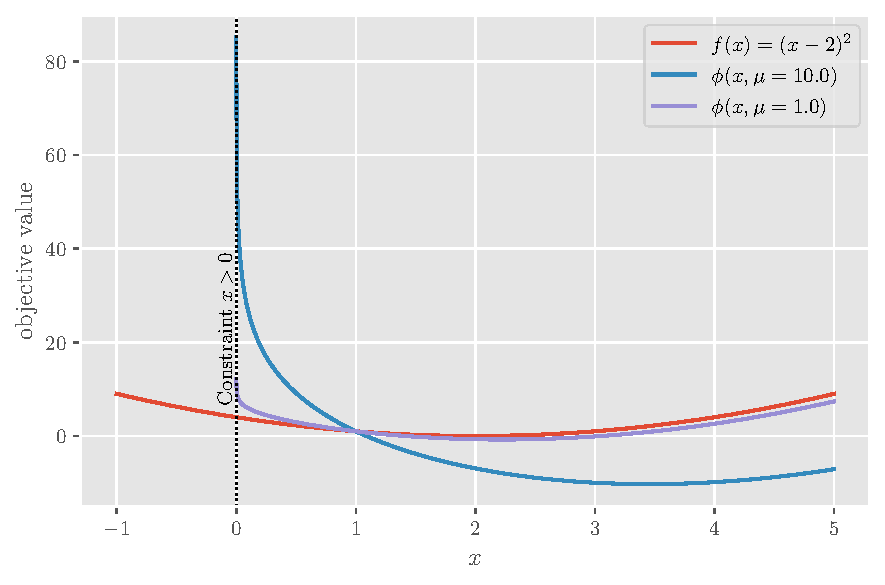
\includegraphics[width=0.6\textwidth]{figs/optimization/barrier.pdf}
    \caption{Logarithmic barrier for the constraint $x>0$: plots of $f(x)=(x-2)^2$ and $\phi(x,\mu)=f(x)-\mu\log x$ ($\mu\in\{10,1.0\}$). The barrier diverges as $x\to0^+$, so smaller $\mu$ more closely tracks $f$ while keeping iterates in the interior.}
    \label{fig:barrier}
\end{figure}


\begin{exampleBox}
    \textbf{Example}:
    Consider the problem:
    \begin{equation}
    \begin{aligned}
    \min_{x_1, x_2} \quad & f(x_1, x_2) = x_1^2 + 10x_2^2 \\
    \text{subject to} \quad & h(x_1, x_2) = 1 - (x_1 - 2)^2 - (x_2 - 2)^2 \ge 0
    \end{aligned}
    \end{equation}
    The objective function's minimum is at $(0,0)$, but the constraint is a circular region centered at $(2,2)$ with a radius of 1, which doesn't contain the unconstrained minimum. The solution must therefore lie on the boundary of the circle.

    The barrier problem is
    \begin{equation}
    \min_{x_1, x_2} \quad \phi(\mathbf{x}, \mu) = (x_1^2 + 10x_2^2) - \mu \log\left(1 - (x_1 - 2)^2 - (x_2 - 2)^2\right)
    \label{eq:barrier-problem-example}
    \end{equation}

    We can solve this using Newton's method. The core of the MATLAB code would look like this:

    \begin{verbatim}
    % Define objective and constraint functions, plus their gradients and Hessians
    f = @(x) x(1)^2 + 10*x(2)^2;
    grad_f = @(x) [2*x(1); 20*x(2)];
    H_f = @(x) [2, 0; 0, 20];

    h = @(x) 1 - (x(1)-2)^2 - (x(2)-2)^2;
    grad_h = @(x) [-2*(x(1)-2); -2*(x(2)-2)];
    H_h = @(x) [-2, 0; 0, -2];

    % Define the barrier objective and its derivatives
    phi = @(x, mu) f(x) - mu * log(h(x));
    grad_phi = @(x, mu) grad_f(x) - (mu/h(x)) * grad_h(x);
    H_phi = @(x, mu) H_f(x) - (mu/h(x))*H_h(x) + (mu/h(x)^2)*grad_h(x)*grad_h(x)';

    % Initial guess (must be strictly feasible)
    x = [2; 2];

    % Loop over decreasing mu values
    for mu = [1:-0.001:0.001]
        % Newton's method to minimize phi for the current mu
        while norm(grad_phi(x, mu)) > 1e-8
            x = x - H_phi(x, mu) \ grad_phi(x, mu);
        end
    end
    \end{verbatim}

    As we decrease $\mu$, the solution to the barrier problem traces a path from the ``analytic center'' of the feasible region toward the true constrained optimum on the boundary. \autoref{fig:barrier-example} shows the solution path for $\mu\in\{10,0.001\}$. The final solution found by the algorithm is the point on the circle closest (in a weighted sense) to the unconstrained minimum at $(0,0)$ and corresponds to $\mu=0.001$.

    \begin{figure}[H]
        \centering
        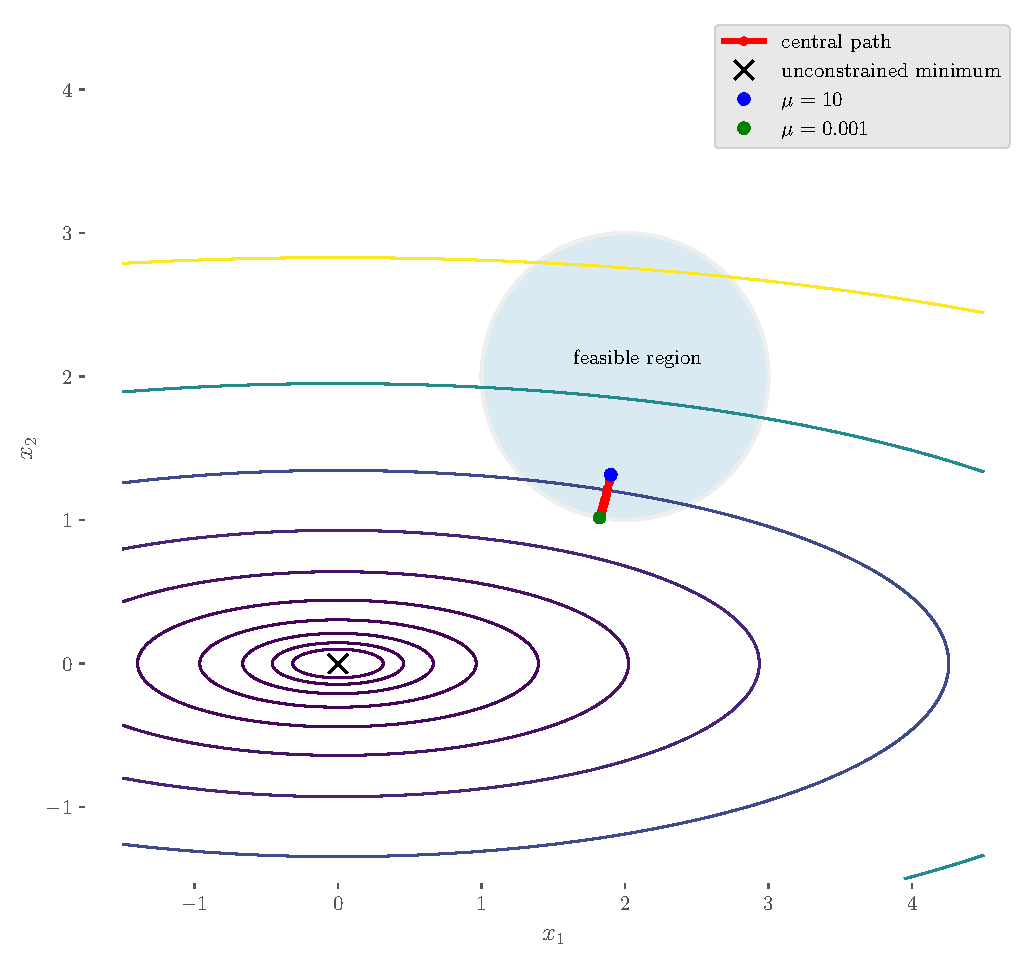
\includegraphics[width=0.6\textwidth]{figs/optimization/barrier_example.pdf}
        \caption{Solution path for the barrier problem \autoref{eq:barrier-problem-example}: $\mu\in\{10,0.001\}$.}
        \label{fig:barrier-example}
    \end{figure}

\end{exampleBox}


\section{\texorpdfstring{Mixed-Integer Optimization\textsuperscript{*}}{Mixed-Integer Optimization}}
\label{sec:mixed-integer-optimization}

We now move into a class of optimization problems where the feasible set $\mathcal{D}$ is no longer a continuous region within $\mathbb{R}^N$. Many engineering decisions are not continuous but discrete. For example, we might need to decide which molecular species to include in a reaction, whether a reactor is on or off, the exact number of trays in a distillation column, or any decision that can be framed as a ``yes'' or ``no'' choice. When the decision variables $\mathbf{x}$ are restricted to discrete values, we have an integer problem. If the problem involves a mix of both discrete and continuous variables, it is called a \textbf{mixed-integer problem}.

One might initially think that because the feasible set of integers $\mathbb{Z}^N$ is smaller than the set of real numbers $\mathbb{R}^N$, these problems should be easier. Unfortunately, the opposite is true. Mixed-integer problems are notoriously difficult and are generally classified as NP-hard. This comes from a combinatorial explosion. Consider designing a 10-amino-acid peptide where there are 20 possible amino acids for each position. This creates $20^{10}$ different possible peptide sequences, a number far too large to check one by one.

The difficulty is that we have lost the smooth landscape that guided our continuous methods: neighboring integer points can have very different objective values, so gradients are not informative. A common approach is to temporarily drop the integrality requirements and solve the resulting continuous problem; this is called a \emph{relaxation}. The relaxation is easier to solve, and its objective value is optimistic for the objective (``too good to be true'') serving as a lower bound in minimization and an upper bound in maximization. However, taking the relaxed solution and simply rounding the integer variables is rarely reliable, as rounded points may violate constraints or be far from optimal. Instead, relaxations are used as building blocks inside exact algorithms such as branch-and-bound (and variants like branch-and-cut) to compute bounds and systematically prove optimality, and inside heuristics to generate good candidates. In 10.34, we will focus on branch-and-bound and use relaxations primarily for bounding rather than as standalone solutions.

\subsection{\texorpdfstring{Branch and Bound\textsuperscript{*}}{Branch and Bound}}
\label{sec:branch-and-bound}

Since brute-force checking every possibility is out of the question, we need a more intelligent strategy. While stochastic methods like simulated annealing exist, the most widely used exact framework for these problems is \textbf{branch and bound}. The goal of branch and bound is to perform an exhaustive search implicitly, meaning it explores the entire space of possibilities while evaluating as few of them as possible. Its power comes from the ability to find and compare lower and upper bounds on the optimal solution.

First, we introduce the concept of the relaxed problem. For an integer problem where variables must be, for example, either 0 or 1 ($\mathbf{x} \in \{0, 1\}^N$), we can define a relaxed version where the variables can take any continuous value between 0 and 1 ($\mathbf{x} \in [0, 1]^N$):
\begin{equation}
    { \everymath={\displaystyle}
    \begin{array}{c@{\qquad\qquad}c}
        \min_{\mathbf{x} \in \{0, 1\}^N} f(\mathbf{x}) & \min_{\mathbf{x} \in [0, 1]^N} f(\mathbf{x}) \\[6pt]
        \text{(original problem)} & \text{(relaxed problem)}
    \end{array}
    }
\end{equation}

Because the feasible set of the relaxed problem is larger than the integer one, its optimal objective value provides a powerful piece of information: it is a lower bound on the best possible value for the original integer problem. This is because for minimization, enlarging the feasible set cannot increase the optimal value (it can only decrease or leave it unchanged).

The branch and bound algorithm uses this idea to build a search tree. The first step is to \textbf{branch}. We take the original problem and split it into two or more subproblems. For a binary variable $x_1$, we would create one subproblem where $x_1$ is fixed to 0 and another where $x_1$ is fixed to 1. This divides the search space.

The second step is to \textbf{bound}. For each of these new nodes in our search tree, we calculate a lower and an upper bound on the best possible solution within that branch. (For minimization problems, the relaxation's objective value is a lower bound and any feasible integer solution gives an upper bound; for maximization, the directions are reversed.) The lower bound is found by solving the continuous relaxation of the subproblem. For the node where $x_1=0$, we would solve the problem with $x_1$ fixed at 0 and all other variables relaxed to be in $[0,1]$. The upper bound is established by finding any valid integer solution in that branch. The best feasible integer solution found so far across the entire tree serves as the global upper bound for the whole problem.

The third and most important step is to \textbf{fathom}, or prune, the tree. This is where the efficiency comes from. If we find that the lower bound of a particular node is higher than our current best global upper bound, we can completely discard that node and its entire subtree. There is no need to explore it further because we are guaranteed that no integer solution in that entire branch can ever be better than the integer solution we have already found. This allows us to cut away vast portions of the combinatorial search space without ever looking at them.

The algorithm proceeds by repeatedly branching on variables, calculating bounds for the new subproblems, and fathoming branches until the entire space has been implicitly covered. The best integer solution found during this process is the global optimum.

\begin{exampleBox}
    \textbf{Example: Branch-and-Bound (Minimization).}
    Imagine a simple graph: a triangle with three vertices (1, 2, and 3) and the three edges connecting them ((1,2), (2,3), and (1,3)). Our goal is to solve the minimum vertex cover problem on this graph. This means we want to find the smallest set of vertices such that every single edge is touched by at least one selected vertex.
    
    We can frame this as a 0-1 integer program. Let's define a binary variable $x_i \in \{0, 1\}$ for each vertex $i$. We'll set $x_i=1$ if we decide to include vertex $i$ in our cover, and $x_i=0$ otherwise. Formally, we write the problem as
    \begin{equation}
    \begin{aligned}
    \min\ z &= x_1+x_2+x_3\\
    \text{s.t. }& x_1+x_2\ge 1,\quad x_2+x_3\ge 1,\quad x_1+x_3\ge 1,\\
    & x_i\in\{0,1\}\ (i=1,2,3)
    \end{aligned}
    \end{equation}    
    Now, we begin by relaxing the integrality constraints. Replace $x_i\in\{0,1\}$ by $0\le x_i\le 1$. Summing the three covering constraints gives
    \begin{equation}
    (x_1{+}x_2)+(x_2{+}x_3)+(x_1{+}x_3) \ge 3
    \quad\Longrightarrow\quad
    2(x_1{+}x_2{+}x_3) \ge 3
    \end{equation}
    so any feasible continuous point satisfies $x_1{+}x_2{+}x_3\ge \tfrac{3}{2}$. By symmetry, the continuous optimum is
    \begin{equation}
        \mathbf{x}^\star_{\mathrm{cont}}=\left(\frac{1}{2},\frac{1}{2},\frac{1}{2}\right) \quad \text{with} \quad z_{\mathrm{cont}}=\frac{3}{2}
    \end{equation}
    Because this is a minimization problem, every continuous optimal value is an LB on the true integer optimum. Next, we branch on the fractional variable $x_1$. We create two subproblems: one where $x_1=0$ and one where $x_1=1$.
    
    For the left child ($x_1=0$), the constraints $x_1{+}x_2\ge 1$ and $x_1{+}x_3\ge 1$ become $x_2\ge 1$ and $x_3\ge 1$. With $0\le x_i\le 1$, this forces $x_2=x_3=1$, so the node is already integral: $\mathbf{x}=(0,1,1)$ with $z=2$. This becomes the best known integer solution (incumbent), so the current global upper bound is 2, and thus \(z^\star \le 2\).
    
    For the right child ($x_1=1$), the constraints $x_1{+}x_2\ge 1$ and $x_1{+}x_3\ge 1$ are redundant; the remaining condition is $x_2{+}x_3\ge 1$ with $0\le x_i\le 1$. The continuous relaxation has optimal value $z_{\mathrm{cont}}=2$ (achieved, for example, by $x_2=x_3=\tfrac12$). This node also contains integer solutions $(1,1,0)$ and $(1,0,1)$ with the same objective $2$. Since the node LB equals the current global UB ($2$), we prune by bound.

    
    Now, we have a best-known integer solution $\mathbf{x}=(0,1,1)$ with $z=2$. Every open subtree is either infeasible, integral, or has LB $\ge 2$. Thus, no better solution exists and $z^\star=2$ is globally optimal.
    
    % -------- Node text (top part = model snapshot; bottom part = small status line) --------
    {
    \def\rootMIP{$\min\ x_1{+}x_2{+}x_3$\\
    subject to\\
    \hspace{0.6em}$x_1{+}x_2\ge 1$\\
    \hspace{0.6em}$x_2{+}x_3\ge 1$\\
    \hspace{0.6em}$x_1{+}x_3\ge 1$\\
    \hspace{0.6em}$x_i\in\{0,1\}$}
    
    \def\rootLP{$\min\ x_1{+}x_2{+}x_3$\\
    subject to (continuous relaxation)\\
    \hspace{0.6em}$x_1{+}x_2\ge 1$,\ $x_2{+}x_3\ge 1$\\
    \hspace{0.6em}$x_1{+}x_3\ge 1$,\ $0\le x_i\le 1$\\
    \nodepart{two}
    {\scriptsize $\mathbf{x}^\star_{\mathrm{cont}}=(\tfrac12,\tfrac12,\tfrac12)$,\ $z_{\mathrm{cont}}=\tfrac32$ (continuous relaxation)}
    }
    
    \def\nodeLeft{$x_1=0$ subproblem\\
    $\Rightarrow$ constraints force $x_2=1,\ x_3=1$\\
    \nodepart{two}
    {\scriptsize integral: $\mathbf{x}=(0,1,1)$,\ $z=2$ $\Rightarrow$ best known integer solution $z^\star=2$}
    }
    
    \def\nodeRight{$x_1=1$ subproblem\\
    Constraints $x_1{+}x_2\ge1$ and $x_1{+}x_3\ge1$ are redundant;\\
    remaining: $x_2{+}x_3\ge1$, $0\le x_i\le1$\\
    \nodepart{two}
    {\scriptsize Continuous optimum $z_{\mathrm{cont}}=2$ (e.g., $x_2{=}x_3{=}\tfrac{1}{2}$).\\
    LB $=2 \ge$ UB $=2$ $\Rightarrow$ prune by bound}
    }
    
    \tikzset{
      > =Latex,
      parent node/.style={
        rectangle split,
        rectangle split parts=2,
        align=left,
        text width=5.2cm,
        draw,
        rounded corners,
        node distance=1.1cm and 0.3cm
      }
    }
    

    \begin{center}
    \begin{tikzpicture}
    \node[parent node,rectangle split parts=1] (A) {\rootMIP};
    \node[parent node,below=of A] (B) {\rootLP};
    \node[parent node,below left =of B, xshift=2cm] (C) {\nodeLeft};
    \node[parent node,below right=of B, xshift=-2cm] (D) {\nodeRight};
    
    \draw[->] (A.south) -- (B.north)
      node[midway,right] {\scriptsize solve continuous relaxation};
    
    \draw[->] (B.south) -- ++(0,-0.6) -| (C.north)
      node[near end,left] {\scriptsize branch: $x_1=0$};
    
    \draw[->] (B.south) -- ++(0,-0.6) -| (D.north)
      node[near end,right] {\scriptsize branch: $x_1=1$};
    \end{tikzpicture}
    \end{center}
    }
\end{exampleBox}
    
It is worth noting that modern MILP/MINLP solvers further strengthen the relaxation with \emph{branch-and-cut}: at each node they derive and add valid inequalities (``cuts''), such as cover, clique, flow/disjunctive, or lift-and-project cuts, to eliminate fractional solutions and improve the bound before deciding to branch. Branch-and-cut is especially effective for 0-1 models where strong, problem-specific cuts are available (e.g., network design, facility location, set covering, routing). For completeness, another common variant is \emph{branch-and-price}, which couples branch-and-bound with column generation and is used when the natural formulation has exponentially many variables (crew scheduling, vehicle routing, etc.).

We conclude this section by observing that the entire strategy of branch-and-bound hinges on our ability to efficiently solve the continuous, relaxed problems that provide lower bounds. Branch-and-bound is most effective when these relaxations are convex because we can compute tight global lower bounds quickly. For nonconvex MINLPs, global solvers typically use \emph{spatial} branch-and-bound together with convex underestimators/relaxations to obtain valid bounds; however, constructing and tightening these relaxations can itself be NP-hard and often requires substantial additional branching and cutting, which is why such problems scale much more poorly. Suffice it to say that modern solvers are quite sophisticated and can handle a wide range of problems. The field of optimization is vast and complex, and we are only scratching the surface here.

\section{\texorpdfstring{Gradient-Free Optimization\textsuperscript{*}}{Gradient-Free Optimization}}
\label{sec:gradient-free-optimization}


Throughout our discussion, we have relied on a crucial piece of information: the gradient $\nabla f(\mathbf{x})$, and often the Hessian $\nabla^2 f(\mathbf{x})$. These derivatives guided our search for a minimum. But what if we do not have access to them? This situation is common when the objective function $f(\mathbf{x})$ is the result of a complex simulation or a physical experiment, where the underlying mathematical model is unknown or too complex to differentiate. This gives rise to a field also known as \textbf{derivative-free} or \textbf{black-box optimization}. The methods used are sometimes called \textbf{zero-th order methods} because they only use function values (zero-th order information), not derivatives.

One option is to estimate the gradient numerically using finite differences, but this can be very computationally expensive and may introduce significant numerical error. A better approach is often to use an algorithm specifically designed for a derivative-free setting.

\subsection{\texorpdfstring{The Nelder-Mead Method\textsuperscript{*}}{The Nelder-Mead Method}}
\label{sec:nelder-mead-method}

A classic and widely used gradient-free algorithm is the \textbf{Nelder-Mead method}. Instead of following a gradient, this method explores the search space using a geometric object called a simplex. A simplex is the generalization of a triangle to arbitrary dimensions: in one dimension it is a line segment, in two dimensions it is a triangle, and in three dimensions it is a tetrahedron. In an $N$-dimensional space, a simplex is formed by $N+1$ vertices.

\begin{center}
\resizebox{.6\textwidth}{!}{
\begin{tikzpicture}[
    dot/.style={circle,fill=black,inner sep=1.8pt},
    thick, line join=round, line cap=round
  ]
  % --- helpers
  \def\R{2.1}            % half-size of each gray square
  \def\dx{5.4}           % horizontal spacing between panels
  
  % ===== Panel 1: point =====
  \begin{scope}[shift={(0,0)}]
    \fill[white!15] (-\R,-\R) rectangle (\R,\R);
    \node[dot] at (-.35,-.15) {};
    % \node at (0,-2.5) {$N=0$};
  \end{scope}
  
  % ===== Panel 2: segment =====
  \begin{scope}[shift={(\dx,0)}]
    \fill[white!15] (-\R,-\R) rectangle (\R,\R);
    \coordinate (P1) at (-1.2,-.25);
    \coordinate (P2) at ( 1.25,-.25);
    \draw (P1) -- (P2);
    \node[dot] at (P1) {};
    \node[dot] at (P2) {};
    % \node at (0,-2.5) {$N=1$};
  \end{scope}
  
  % ===== Panel 3: filled triangle =====
  \begin{scope}[shift={(2*\dx,0)}]
    \fill[white!15] (-\R,-\R) rectangle (\R,\R);
    \coordinate (A) at (-1.25,-.95);
    \coordinate (B) at ( 1.25,-.95);
    \coordinate (C) at ( 0,1.25);
    \fill[blue!35,opacity=.45] (A)--(B)--(C)--cycle;
    \draw (A)--(B)--(C)--cycle;
    \node[dot] at (A) {};
    \node[dot] at (B) {};
    \node[dot] at (C) {};
    % \node at (0,-2.5) {$N=2$};
  \end{scope}
  
  % ===== Panel 4: tetrahedron =====
  \begin{scope}[shift={(3*\dx,0)}]
    \fill[white!15] (-\R,-\R) rectangle (\R,\R);
  
    % vertices
    \coordinate (T) at ( .55, 1.55);
    \coordinate (L) at (-1.35,-.35);
    \coordinate (B) at ( 1.00,-1.35);
    \coordinate (R) at ( 1.85, .15);
  
    % faces
    \fill[blue!35,opacity=.45] (L)--(B)--(T)--cycle;      % left/front face
    \fill[blue!35,opacity=.45] (T)--(B)--(R)--cycle;      % right face
  
    % visible edges
    \draw (L)--(B)--(T)--cycle;
    \draw (T)--(B)--(R)--cycle;
  
    % hidden edge
    \draw[dashed] (L)--(R);
  
    % vertices
    \node[dot] at (T) {};
    \node[dot] at (L) {};
    \node[dot] at (B) {};
    \node[dot] at (R) {};
    % \node at (0,-2.5) {$N=3$};
  \end{scope}
\end{tikzpicture}
}
\end{center}

The algorithm begins with an initial simplex in the search space. At each iteration, it evaluates the objective function at all $N+1$ vertices and identifies the worst vertex (highest objective value), the best vertex (lowest value), and the second-worst vertex. The goal is to replace the worst point with a new, better point located by moving ``downhill''. This is achieved through a series of adaptive moves. The primary move is \textbf{reflection}, where the worst point is flipped through the centroid of the remaining points. If this new point is better, the algorithm might get optimistic and try an \textbf{expansion} to stretch the simplex even further in this promising direction. If the reflected point is still poor, the algorithm performs a \textbf{contraction}, pulling the point back towards the other vertices to search more locally. If even contraction fails, the simplex performs a \textbf{shrink} move, pulling all points closer to the single best vertex.

\begin{figure}[H]
    \centering
    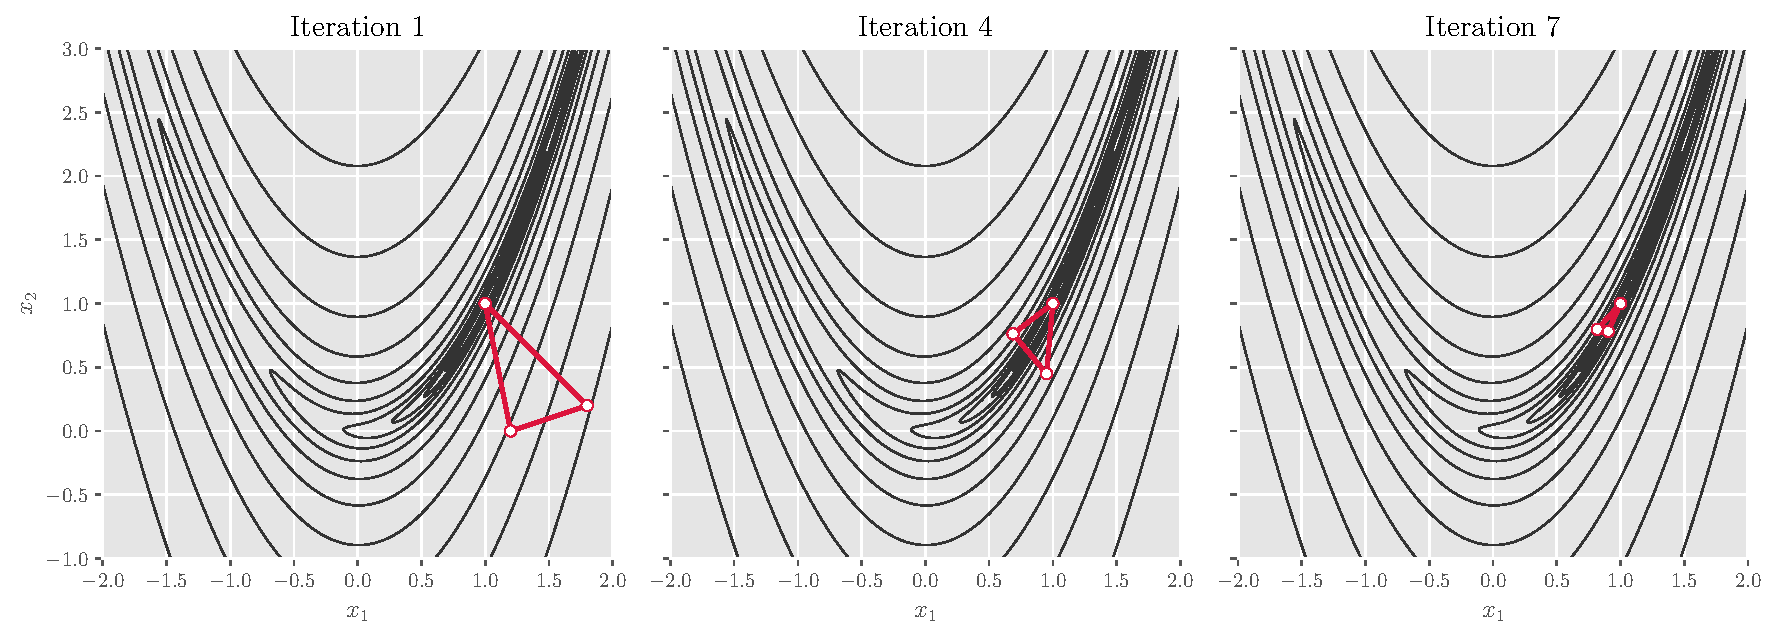
\includegraphics[width=0.9\textwidth]{figs/optimization/nelder_mead_3panel.pdf}
    \caption{Three snapshots (iterations 1, 4, and 7) of the Nelder-Mead method on the 2D Rosenbrock function. Contours show level sets of $f(x_1,x_2)$; the red triangle is the simplex. At each step the worst vertex is replaced via reflection/expansion/contraction, causing the simplex to translate and shrink along the curved valley toward the minimizer at $(1,1)$.}
    \label{fig:nelder-mead-3d}
\end{figure}

Through this sequence of reflections, expansions, and contractions, the simplex tumbles and morphs its way across the landscape of the objective function, gradually crawling downhill toward a minimum. The ability of the simplex to grow and shrink gives the method a built-in notion similar to a trust region, allowing it to adapt its search scale. The Nelder-Mead method often performs remarkably well for problems with low dimensionality, typically in the range of 2 to 8 dimensions. However, it does not scale well to high-dimensional problems, as the simplex becomes an increasingly inefficient tool for exploring a space whose volume grows exponentially with dimension---a classic example of the curse of dimensionality.

\textbf{Convergence and practicalities.}\quad
The classical Nelder-Mead method has no general convergence guarantee in dimension $\ge 2$ for smooth objectives. Smooth counterexamples exist where it converges to a nonstationary point. Positive results hold only in special cases, like strictly convex 1D problems with bounded level sets and certain restricted 2D variants, and do not cover typical nonconvex, higher-dimensional settings. In practice, performance relies on a few basics: rescale variables; use both a simplex-size and a function-decrease tolerance for stopping; watch for degeneracy or stalling and consider restarts or re-expansions; be cautious with noise or discontinuities; handle constraints via penalties, projections, or box-aware variants; and note that effectiveness degrades as dimension grows. Beyond roughly $N\gtrsim 10$, trust-region or model-based derivative-free solvers (and quasi-Newton methods when gradients or reliable finite differences are available) typically scale better.

\section{Optimization: A Summary}

We have now surveyed some of the most fundamental concepts and algorithms in numerical optimization. The general problem is always of the form $\min_{\mathbf{x} \in \mathcal{D}} f(\mathbf{x})$, but the choice of method depends heavily on the nature of the feasible set $\mathcal{D}$ and the information available about the objective function $f$.

When the problem is unconstrained, meaning $\mathcal{D} = \mathbb{R}^N$ (or, more generally, $\mathcal{D}$ coincides with the natural domain of $f$), we can use gradient information to find a solution. Steepest descent offers the simplest approach, moving in the direction of the negative gradient at each step. While guaranteed to converge under mild conditions, this method can be quite slow, particularly near the solution. Newton's method addresses this limitation by incorporating second-order information through the Hessian matrix, leading to much faster convergence when close to the optimum. However, computing and inverting the Hessian at each iteration can be computationally expensive. Quasi-Newton methods like BFGS provide an attractive middle ground, building up an approximation to the Hessian using only gradient information from previous iterations.

The presence of constraints changes the optimization landscape. For equality constraints of the form $\mathbf{g}(\mathbf{x}) = 0$, the method of Lagrange multipliers transforms the constrained problem into finding critical points of the Lagrangian:
\begin{equation}
    L(\mathbf{x}, \boldsymbol{\lambda}) = f(\mathbf{x}) - \boldsymbol{\lambda}^T \mathbf{g}(\mathbf{x})
\end{equation}
This reduces the problem to solving the system $\nabla_{\mathbf{x}} L = 0$ and $\mathbf{g}(\mathbf{x}) = 0$, which can be tackled using Newton's method for systems of equations.

Inequality constraints require different techniques since the active set (the constraints that are binding at the solution) is unknown \emph{a priori}. Interior-point methods handle this by introducing a barrier function that prevents iterates from leaving the feasible region. The constrained problem is then solved as a sequence of unconstrained barrier problems with the barrier parameter gradually reduced to recover the original problem.

When decision variables must take discrete values, we enter the world of integer programming. These problems are fundamentally harder due to the combinatorial nature of the search space. Branch-and-bound provides a systematic enumeration strategy, using bounds on subproblems to eliminate large portions of the search tree without explicitly evaluating every possibility.

Finally, when gradient information is unavailable, whether due to noisy function evaluations, discontinuities, or computational constraints, gradient-free methods become necessary. The Nelder-Mead simplex algorithm is one example of such a method, using only function values at a collection of points to guide the search toward better solutions.

%%% Local Variables:
%%% mode: LaTeX
%%% TeX-master: "../main"
%%% End: